\documentclass[../../main.tex]{subfiles}

% Image numbers: 10-201 inclusive

\begin{document}

\newchapter{Design Process}{design-process}

\section{Initial designs} \label{sec:design-process:initial-designs}

\subsection{Operation and initial constraint analysis} \label{sec:design-process:initial-designs:operation-and-initial-constraint-analysis}

Initially an analysis based on estimated parameters was performed, using a normal distribution around each parameter to form a search space of data in which to find the most likely power requirement in order to find an early motor size and decide parameters such as wingspan and aspect ratio. 

The cruise speed was estimated using preliminary values of mass, $C_L$, aspect ratio, and span. The function is shown in Appendix B.
This function could then be used to form a probability distribution and find the most likely value of the cruise velocity based on the estimated values.
The probability distribution is shown in Figure 2.

We find that the mean and median both have values of approximately 21m/s, and so this taken as the estimated cruise velocity at this point. 

The power requirements can then be estimated using a similar procedure, taking preliminary values for efficiency, mass, Vcruise (as estimated above), $C_L$, and $C_D$, again using normal distributions of values for the unknowns.
Appendix B contains the function used.
This can then be used to find the probability distribution for the power required in cruise, shown in Figure 4.

\begin{figure}[H]
    \centering
    \begin{subfigure}[b]{0.49\columnwidth}
        \centering
        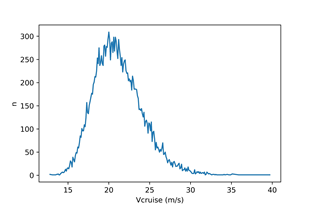
\includegraphics[width=\textwidth]{cruise-velocity-distribution}
        \caption{Velocity}
        \label{fig:cruise-distribution:velocity}
    \end{subfigure}
    \hfill
    \begin{subfigure}[b]{0.49\columnwidth}
        \centering
        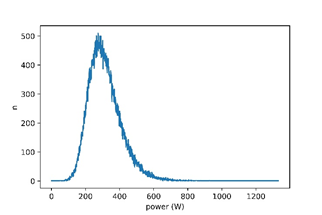
\includegraphics[width=\textwidth]{cruise-power-distribution}
        \caption{Power}
        \label{fig:cruise-distribution:power}
    \end{subfigure}

    \caption{expected distribution of selected properties during cruise.}
    \label{fig:cruise-distribution}
\end{figure}

We find that the mean value of the power required in cruise is 315W, with a median of 302W, giving an estimated power requirement in cruise of around 310W.
There is more uncertainty with this than with the cruise speed due to the larger range of values covered within one standard deviation of the mean, however this still provides a good starting point for the project.

\subsection{Further constraint analysis} \label{sec:design-process:initial-designs:further-constraint-analysis}

Using the refined parameters found in the initial constraint analysis, design decisions made, and further analysis of the UAV, the constraint analysis can be combined to show all parts of the flight profile to find the minimum power requirement.
This code gives more refined estimates for the power requirement in different areas of the flight envelope, as well as take-off speed.
This can be updated quickly and easily as design decisions are made and various operational parameters are refined.
Figure 5 shows the final plots after all research and design decision were made.

\importimage{full-constraint-analysis}{full constraint analysis plot with feasible region highlighted.}{Full constraint analysis}{0.85}
\importimage{takeoff-speed-plot}{takeoff speed plot.}{Takeoff speed plot}{0.85}

It can be seen that the lowest thrust to weight ratio required is around 0.29, which corresponds to a power requirement of around 520W, however this is for a wing loading of only 100N/m2.
The final wing loading of ELMO UAV turned out to be approximately 111N/m2, giving a thrust to weight requirement of just over 0.3 and a corresponding power requirement of around 650W, and so the final selection of motors is sufficient with a small amount of power to spare. 

\subsection{Wing} \label{sec:design-process:initial-designs:wing}

Early in the project, due to its nature: the complexity of certain components and the limited budget, it was decided that a simple rectangular wing would be used on the UAV.
Taking the modularity onto account, a rectangular wing would reduce the possible number of engine housing units needed, therefore reducing the amount of design and manufacturing, and therefore cost of the project. 

The UAV had a 2m span, with a fixed chord of 30cm, which gave an aspect ratio of 6.6.
The chord length was initially at 25cm, closer to the desired aspect ratio of 8.
However, concerns regarding the size of flaps and ailerons were raised as a significant amount of the wingsipan would be lost to the motor housing units, so the chord length was increased to 30cm as a compromise.  

Once a wing shape had been decided a more detailed analysis of possible airfoil sections took place.
Initial 2D simulations were run on XFLR (XFLR, 2019) to narrow the choice down to five airfoils.
The analysis was run at a Reynolds number of $1.35x10^6$, calculated using standard atmospheric conditions at a cruise speed of 20m/s and a reference length on XFLR of 1m. 

Although the purpose of the project is to improve the efficiency of electric aircraft by altering the position of the propulsion units, the aim is not to produce the most efficient aircraft, but more a test craft which can be reused.
Therefore, when choosing the airfoil the main considerations where not only L/D but also stall angle, max Cl and moment coefficient amongst others.
The analysis narrowed down to four potential airfoils: The Clark Y, S1223, NACA6412, RG15A213, whose coordinates were taken from (Tools, 2019) Figures 1a,b, and c  show the Cl-alpha, Cl/Cd, and Cm – alpha curves respectively of four suitable airfoils. 

The Clark Y (blue line) is very common among model UAV makers because of its gentle stall angle at around 12 degrees, with a further sharper drop off at around 20degrees.
It also has a gentle moment coefficient which makes it stable to changes in attitude during flight. 

The S1223 (black line) has an extremely high L/D ratio due to its high camber, it also has a slightly higher stall angle than the Clark Y (at around 14 degrees).
However, it has an unfavourably large moment coefficient, which may make it unstable in flight.
Its high camber and narrow trailing edge may also make it difficult to implement high lift devices as well as it not being strong enough to support a tractor propulsion set up. 

The NACA6412  (green line) has a high L/D ratio up to 10degrees of incidence as well as a higher Cl-alpha curve which is useful as a large part of the wing wetted area will be taken by motor housing.
However, it has a slightly higher moment coefficient than the Clark Y at low angle as well a lower, yet gentle, stall angle of 11 degrees.

The RG15A213 (red line) has the lowest Cl – alpha of the five, but has a higher stall angle at 15 degrees as well as having the lowest moment coefficient.

Of the five airfoils above, further analysis would be carried out on the Clark y and the NACA6412 airfoils as they provided good lift performance, strong lift to drag ratio and a manageable moment coefficient.

\importimage{alpha-characteristics}{variation of $C_L$, $C_L/C_D$, and $C_M$ with $\alpha$.}{Angle of attack characteristics}{0.9}

\subsection{Fuselage} \label{sec:design-process:initial-designs:fuselage}

This project is designed with the intention of using electric propulsion on commercial aircraft in the future.
Therefore, the design of the UAV was based around commercial aircraft, this discounted any lightweight or double fuselage seen on many UAV’s such as SPOTTER (SPOTTER, 2019). 

Initial designs included a square, circular and airfoil shaped fuselage.

\importtable{| >{\raggedright\arraybackslash}p{0.12\columnwidth} | >{\raggedright\arraybackslash}p{0.36\columnwidth} | >{\raggedright\arraybackslash}p{0.36\columnwidth} |}{
    \hline
    \textbf{Design} & \textbf{Advantages} & \textbf{Disadvantages} \\
    \hline
    Square & Easy manufacturing and wing attachment; strong structural performance & Poor aerodynamics \\
    \hline
    Circular & Easy to manufacture & Hard to attach wing; difficult to create internal structure \\
    \hline
    Aerofoil & Aerodynamic; aesthetically pleasing & Difficult to manufacture \\
    \hline
}{tradeoffs involved in the type of fuselage design.}{fuselage-tradeoffs}

\importimage{potential-aerofoil-design}{potential aerofoil fuselage design.}{Potential aerofoil design}{0.5}

For the wind tunnel model, it was decided that a hybrid of a square fuselage and an airfoil shaped fuselage would be beneficial.
It was thought that a side profile of a NACA0012 airfoil would reduce drag and increase lift, whilst a square front section would make manufacturing easier.
This would give a combination between an aerodynamic design and ease of manufacturing.  

The NACA0012 was chosen as a suitable airfoil as it would provide enough height to hold all the electronics, as well as enough room to reach in in case needed. 

The initial fuselage design was 1.5m long, with a width of 175mm and a height (at the thickest part) equal to around 180mm. 

\subsection{Tail} \label{sec:design-process:initial-designs:tail}

Note, for many of the tail and control surface mathematical design processes, details of the equations used are unnecessary for understanding, but for the interested reader, they can been seen in the appendices, and appropriately headed and labelled. 

The tail was designed with a volume coefficient process.
First, volume coefficients were estimated from Raymer’s book: ‘Aircraft design: A conceptual approach’, table 9.4 (Raymer, 1989), and a value of 0.8 was selected for the horizontal, and 0.07 for the vertical tail volume.
Next values for tail surface aspect ratios were estimated as 5 for the horizontal tail, and 2 for the vertical tail from table 9.1 in (Raymer, 1989).
The formulae for vertical and horizontal tail volume coefficients for tailplane areas were rearranged to obtain the vertical and horizontal tail areas, where then the aspect ratio selected could be used to determine span, and then MAC of the tail surfaces.
Lastly the taper ratio was used to determine root and tip chords of the tail surfaces.
At this stage, no setting angle was determined as the need for this had not been recognised. 

Next, the spars had to be sized for the wind tunnel test.
We were advised by our supervisor, Prof. Keith Towell to size them for 10g loads (Towell, 2019).
A simple mathematical beam model was used to size the spars in the tail as well as the main structural arm.
The horizontal tail spars were modelled as having a 5g (49.05N) load distributed evenly over the semi span.
Based on values for the inner and outer diameters of the spars, length and chosen material stiffness, the tip deflection was found.
The main structural arm was determined by modelling a 10g point load in line with the horizontal spars, and using inner and outer widths instead of diameters, as it was decided this would be a square section to prevent parts rotating around it.

\subsection{Control surfaces, electronics, and avionics} \label{sec:design-process:initial-designs:control-surfaces-electronics-and-avionics}

The initial design was with the first wind tunnel test in mind, and as such made no plans for functional control surfaces, electronics or avionics at this point.
It was hoped that the first test would ‘nail down’ the basics of the fuselage, wing and tail geometry, or show us where changes would be required from our initial design, and subsequent models and tests could validate the performance of more complex aspects of the design and performance of the UAV. 

\subsection{Propulsion} \label{sec:design-process:initial-designs:propulsion}

\subsubsection{Twist-in motor attachment} \label{sec:design-process:initial-designs:propulsion:twist-in-motor-attachment}

\begin{figure}[H]
    \centering
    \begin{subfigure}[b]{0.49\columnwidth}
        \centering
        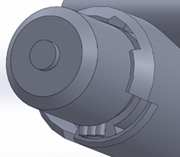
\includegraphics[width=\textwidth]{twist-in-in-place}
        \caption{Motor in-place in housing}
        \label{fig:twist-in:in-place}
    \end{subfigure}
    \hfill
    \begin{subfigure}[b]{0.49\columnwidth}
        \centering
        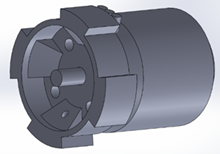
\includegraphics[width=\textwidth]{twist-in-attached}
        \caption{Bracket attached to motor}
        \label{fig:twist-in:attached}
    \end{subfigure}

    \begin{subfigure}[b]{0.49\columnwidth}
        \centering
        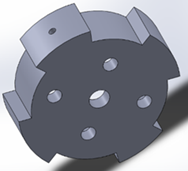
\includegraphics[width=\textwidth]{twist-in-bracket}
        \caption{Bracket}
        \label{fig:twist-in:bracket}
    \end{subfigure}
    \hfill
    \begin{subfigure}[b]{0.49\columnwidth}
        \centering
        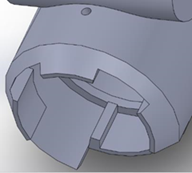
\includegraphics[width=\textwidth]{twist-in-housing}
        \caption{Housing}
        \label{fig:twist-in:housing}
    \end{subfigure}
    \caption{CAD models of the twist-in motor attachment used in the tail.}
    \label{fig:twist-in}
\end{figure}

Designed early on in the project this was a proposed design for the attachment of the wing motors, however when the design criteria changed to include a battery and ESC in the movable propulsion unit, a new design was required.
However, this design is still used in the tail location as the battery and ESC are fixed in the fuselage for that configuration, and so only the motor moves making this an ideal solution.
The design is intended to allow for very quick and simple removal and replacement of the motor when changing configurations of the UAV in order to reduce ground time at the flying days.
This utilises a twist and fix design where four tabs on the bracket, shown in Figure 1 c), which attaches to the back of the motor as shown in Figure 1 b), engage with four tabs in the housing and the motor then rotates up to a limiting piece to align the bracket and housing, shown in Figure 1 d) and a).
The motor is then secured in place using a small grub screw which engages with the bracket through a clearance hole in the top of the housing, as shown in Figure 1 d), providing the resistance to rotation of the motor while the tabs provide the strength in the direction of the force of the motor.
The large cut-out in the housing, shown in Figure 1 d), is to allow room for the wires of the motor when it is being fitted, as they protrude from the rear part of the motor out to the side, shown in Figure 1 a).
On the final design for the tail there is a full routing designed for the wires but that is was not designed here as this housing was intended for the wing, but then not used.

\subsubsection{Sizing} \label{sec:design-process:initial-designs:propulsion:sizing}

Initial sizing started from the constraint analysis power requirement estimations, allowing motors to be selected.
The constraint analysis at this point was suggesting a power requirement of around 600W, and so motors were researched of around this power from a recommended supplier Outlander, and a number of suitable cost effective motors were found for both the fuselage and wing locations, as listed in Figure 1 a).
These were then used to find suitable ESCs, which were recommended for the motors as 60A and 30A, but due to this being the most common part to fail on previous projects due to overloading, a decision was made to oversize the ESCs by 30\% and so 40A and 80A ESCs were selected.
The batteries were then chosen based on the voltage and current requirements of the motors, meaning that they needed to be 4S to provide the required 14.8V, and the capacity initially chosen simply on weight and cost, with the largest capacity shown being the heaviest we could use.
The C value is used to find the max current output of the battery and so this was chosen to ensure a large safety margin between the max of the battery and the max of the motor to reduce any chance of overheating of the battery while in use. 

The motor selection was then refined due to an increase in the power requirement prediction from the constraint analysis due to confirmations in the UAV design, this meant that the motors could be selected as the Tornado Thumper V3 3548/05 and 3530/14 for the fuselage and wing motors respectively.
This meant that the battery capacities could be checked for time of flight based on an estimated 75\% throttle average throughout a flight, this is an overestimate but gives a useful pessimistic estimation of the flight time.
This showed that the smaller capacity batteries would not be enough to provide a suitable flight time in order to record the data we would need while having a margin in the battery to avoid a power cut-out mid-flight.
Along with finalising the battery selection, the propellers could now be researched as shown in Figure 1 b).
This initially required the maximum propeller diameter to be found for the motors, based on the max rpm of the motor, which would give a tip Mach No of the propeller of around 0.7 which would maximise thrust without having large increases in power requirement due to transonic effects at the blade tip.
This was then used to refine an iterative search of the available propellers from APC, a trusted manufacturer by the University.
The advance ratio was found based on the blade diameter, RPM, and a target max flight speed of 25m/s, and then a suitable propeller found in the database that had a power draw similar to that of the max of the motor at the target flight speed and RPM, while providing enough thrust based on estimations of the aircraft drag.
These propellers were then checked after selection at the target cruise speed of 20m/s to ensure that the thrust would be adequate, and to find an estimation of the efficiency in order to further refine the constraint analysis.
The ideal propellers, however, could not be used due to the specific use case of the project, which requires both tractor and pusher configurations to be employed, as well as counter rotating propellers on each wing, and this meant that the propeller would need to have an equivalent pusher propeller.
This meant that the selection of propellers was forced into non-ideal blades, with the fuselage propeller only having one viable option of the APC 12x6E and 12x6EP propellers, and the wing having two options of the 8x6E and 7x5E, which after analysis of thrust data, the 8x6E was chosen to be used in a motor and propeller wind tunnel test to verify that this propeller would be suitable, and to verify the quoted performance data in order to ensure that the 12x6E would also be suitable. 

\section{Physical testing and validation} \label{sec:design-process:physical-testing-and-validation}

\subsection{Wind tunnel test} \label{sec:design-process:interim-design-review:wind-tunnel-test}

\subsubsection{Fuselage} \label{sec:design-process:interim-design-review:wind-tunnel-test:fuselage}

The fuselage was designed around a hollow 1m long and 20mm square aluminium boom as its core structural element.
Around the boom was a foam and poplar plywood structure, similar to the wing. 

The driving force behind the fuselage design was the need to be able to change the setting angle of the wing with ease.
As a result, the metal boom was fixed to four layers of poplar ply ribs which ran the length of the fuselage. 

To allow the wing setting angle to be changed easily three sets of holes ran through the fuselage.
The front hole was a tight fir for the front spar, so it didn’t move.
The middle was a guide for the rear spar to help changing the angle.
The rear set of holes were to secure the wing in place.
This section contained seven holes in total, each 2 degrees apart, meaning the wings angle could be changed form 0 degrees up to 12 degrees. 

\importimage{fuselage-cross-section}{a cross-section of the fuselage, showing the structure and hole layouts.}{Fuselage cross-section}{0.6}

At the rear of the model, on the underside, the middle two ribs contained an attachment point for the wind tunnel.
This was extruded from the model to enable the model to be easily attached and removed from the struts. 

\importimage{laser-cut-plywood}{laser-cut plywood for the fuselage.}{Laser-cut plywood}{0.7}

\subsubsection{Wing} \label{sec:design-process:interim-design-review:wind-tunnel-test:wing}

The wing was constructed using two hollow aluminium spars as the key structural element.
The front spar at quarter chord, the rear spar at half chord, with outer diameters of 15.88mm and 12.7mm, respectively.
Each spar was 2m long and ran tip to tip through the fuselage.
Surrounding the spars was blue Styrofoam, cut from the university foam cutter.
Separating the foam sections were 3mm thick poplar ply ribs, cut on university laser cutter.
Each rib had a unique design and were individually designed and cut.

\importimage{flap-dfx-file}{DFX file of flap rib for the Clark Y aerofoil section, later used for laser cutting.}{Flap DFX file}{0.6}

There were 6 ribs used in each wing half, in locations that would roughly replicate where the motor housing units would be on the final model.
Therefore, the ribs were located either side of the flap and 130mm outboard.
The next rib, located 101mm outboard, was the rib used to connect the model to the wind tunnel.
Therefore, it was made from 6mm birch ply as this provided enough strength to an integral component.
The two final ribs were located at the wing tip and 50mm inboard.

\importimage{underside-of-wing}{the underside of the wing, showing attachment and flap adjustment methods.}{Underside of wing}{0.6}

The thicker birch ply rib, located 700mm outboard of the centre of the aircraft, contained an extrusion with a hole for a M6 bolt to allow easy attachment and removal to the wind tunnel mounts.
It was located at 700mm from the centre of the fuselage as dictated by the wind tunnel capabilities. 

The foam and ribs for each side of each wing were bonded together using epoxy resin but were not bonded to the spars themselves.
This was to allow the wing sections to be removed from the spars during the wind tunnel test. 

The wings were secured to the wing using two 3D printed clamps on each spar. 

\importimage{internal-spar-structure}{Wing section showing the internal spar structure.}{Internal spar structure}{0.6}

\subsubsection{Control surfaces} \label{sec:design-process:interim-design-review:wind-tunnel-test:control-surfaces}

The main purpose for the wind tunnel model was to cement top level parameters such as airfoil section, setting angle, chord length and wingspan.
As a result, the wind tunnel was unpowered, and ailerons not included in the model.
However, it was important to test the effect of a flap on each wing and which airfoil would be more suitable to the addition of a flap. 

Initial research stated that, for a typical low speed UAV, ailerons take up approximately 40\% of the semi-span, in this case 400mm (Sadraey, 2013).
This left the remaining 60\% for flaps.
However, the design at the time was for the motor housing units to have width of approximately 110mm.
There would be two located on each half of the wing, plus a tip mounted motor as well, which had an unknown depth at the time.
Therefore, the flaps were set to a width of 380mm, which would act as a “worst case scenario” approach to the design and would provide each wing section with a strong test. 

The flaps were designed to be changed manually, whilst the model was still attached to the wind tunnel.
The guided either side of the flaps had M2 holes every 5 degrees up to 35 degrees.
As the flap was altered two M2 bolts would secure the flap in place. 

\importimage{flap-mechanism}{close up of the flap mechanism.}{Flap mechanism}{0.6}

\subsubsection{Tail} \label{sec:design-process:interim-design-review:wind-tunnel-test:tail}

With the mathematical modelling complete, a 3D model of the tail surfaces could then be created as reference for building.
This was done by defining the sketch planes that the roots and tip chord aerodynamic profiles would be created on, importing curves of the aerofoil from coordinate files and parametrizing them (chord length and angle of attack) so that they could be manipulated.
Lofted bases were created between the profiles, then additional details such as cut-outs for spars were added.
This was repeated for all three control surfaces, and then simple models of the tail spars and main structural arm created and added to the overall assembly. 

The initial plan was to use the foam cutter to create the tail profiles, however, this proved to be infeasible as the cut-outs for the spars in a thin aerofoil profile (NACA0012) left very little foam in the wall which resulted in the foam melting at the tip where the cutter had to slow down.  

There wasn’t time to redesign the tail because of the upcoming test, so it was decided to laser cut profiles at equally spaced intervals along the tail surfaces and wrap Solarfilm around it.
Geometry was created in CAD using repeated 3mm profiles intersecting the foam geometry, and then non-intersecting geometry deleted to leave the laser cut profiles, which were quickly exported and cut.
Each profile was mounted and bonded to the spar.
Once the glue had cured, Solarfilm was wrapped around the profiles, with the leading and trailing edges stiffened with card.
This was messy but worked, while we resolved to refine the model for the next iteration of the design.  

The tail was mounted on the model using a friction fit with the spars running through the fuselage and main structural arm.
Holes were drilled through these that were intentionally a half millimetre short of the spacing required.
One horizontal tail surface was glued to one spar, and the other to the second, so they would slot together neatly in the model.
The vertical tail surface contained both spars, and simply slotted in all at once. 

\importimage{wind-tunnel-model}{final wind tunnel model.}{Wind tunnel model}{0.8}

\subsubsection{Test plan} \label{sec:design-process:interim-design-review:wind-tunnel-test:test-plan}

The wind tunnel test had a few objectives.
The first was to validate the designs produced so far, ensuring that lifting surfaces could produce sufficient lift and were able to withstand the predicted structural loads.
Assuming these conditions were met, a combination of aerofoil, wing-body angle, and flap-wing angle needed to be found which optimised the objective function (discussed later in more detail).
Data collected during this optimisation would also be used afterwards to alter the design further - estimating the change to lift or drag that could be obtained by changing the size of the flaps - and to validate the accuracy of CFD simulations. 

Five variables were controllable within the wind tunnel: aerofoil, angle between the wing and the fuselage (wing-body angle), angle between the flaps at maximum deflection and the wing (flap-wing angle), angle of attack, and airspeed.
The experiment space created by all of these variables is much larger than would have been feasible to explore fully within one wind tunnel session, and so the testing was split into two phases - cruise and takeoff - and some simplifications were made to enable a subset of the experiment space to be explored while still yielding near-optimal results.

During cruise, some of the variables can be fixed.
Angle of attack is set to 0o, cruise speed is fixed at 20 m.s-1, and flaps will not be extended.
The experiment space now consists of the two aerofoil options and a number of wing-body angle settings for each one, but can be reduced further by assuming that an increase in wing-body angle will always correspond to an increase in drag, and will cause an increase in lift as long as the wing has not stalled.
The objective function for the cruise phase of testing can then be defined as the combination of aerofoil and wing-body angle which minimise drag while producing at least 70 N of lift, and then the wing-body angle can be gradually increased for each aerofoil until the lift exceeds 70 N, at which point the testing for that aerofoil is terminated. 

After the cruise phase of testing has been completed, the optimal aerofoil section and wing-body angle can be held constant for the takeoff phase of testing.
If a takeoff speed of 12 m.s-1 is assumed, the experiment can alter the flap-wing angle and angle of attack (to account for bumps or irregularities in the runway) to find a flap-wing angle which maximises L/D while still providing sufficient lift for takeoff at the minimum takeoff angle and not stalling at the maximum takeoff angle.
Reasonable maximum and minimum takeoff angles can be determined from assumptions about the size and length of the landing gear, and the amplitude of bumps on the takeoff surface.
Varying the angle of attack between these two bounds does not cost an excessive amount of time as, unlike the flap-wing angle, that parameter can be varied without the wind tunnel being turned off. 

This procedure was written up into a testing plan, whose conditions enabled the design space to be suitably explored without taking up too much time.
Care was taken to ensure that the plan was objective and covered all edge cases (barring extreme edge cases, such as no configurations producing the required amount of lift or structural failure, which would require a more thorough redesign of the aircraft) so that the results did not need to be discussed during the course of testing.
As much time as possible could then be spent changing to aircraft between the required configurations; estimates of how long would be needed to vary each parameter were also made.

Provisions were also made for gathering some data to analyse the stability of the model if there was any time left over at the end of these two testing phases.
With the optimal aerofoil section, wing-body angle, and flap-wing angle according to the objective functions described above, forces and moments on the model were measured for a range of airspeeds and angles of attack.
Since both of these parameters are variable without turning off the wind tunnel, a relatively large amount of data can be collected fairly quickly.
Once a suitable amount of data were collected, similar sweeps of the parameter space with the optimal configuration would be made with the tail taken off. 

\subsubsection{Results and analysis} \label{sec:design-process:interim-design-review:wind-tunnel-test:results-and-analysis}

\begin{figure}[H]
    \centering
    \begin{subfigure}[b]{0.49\columnwidth}
        \centering
        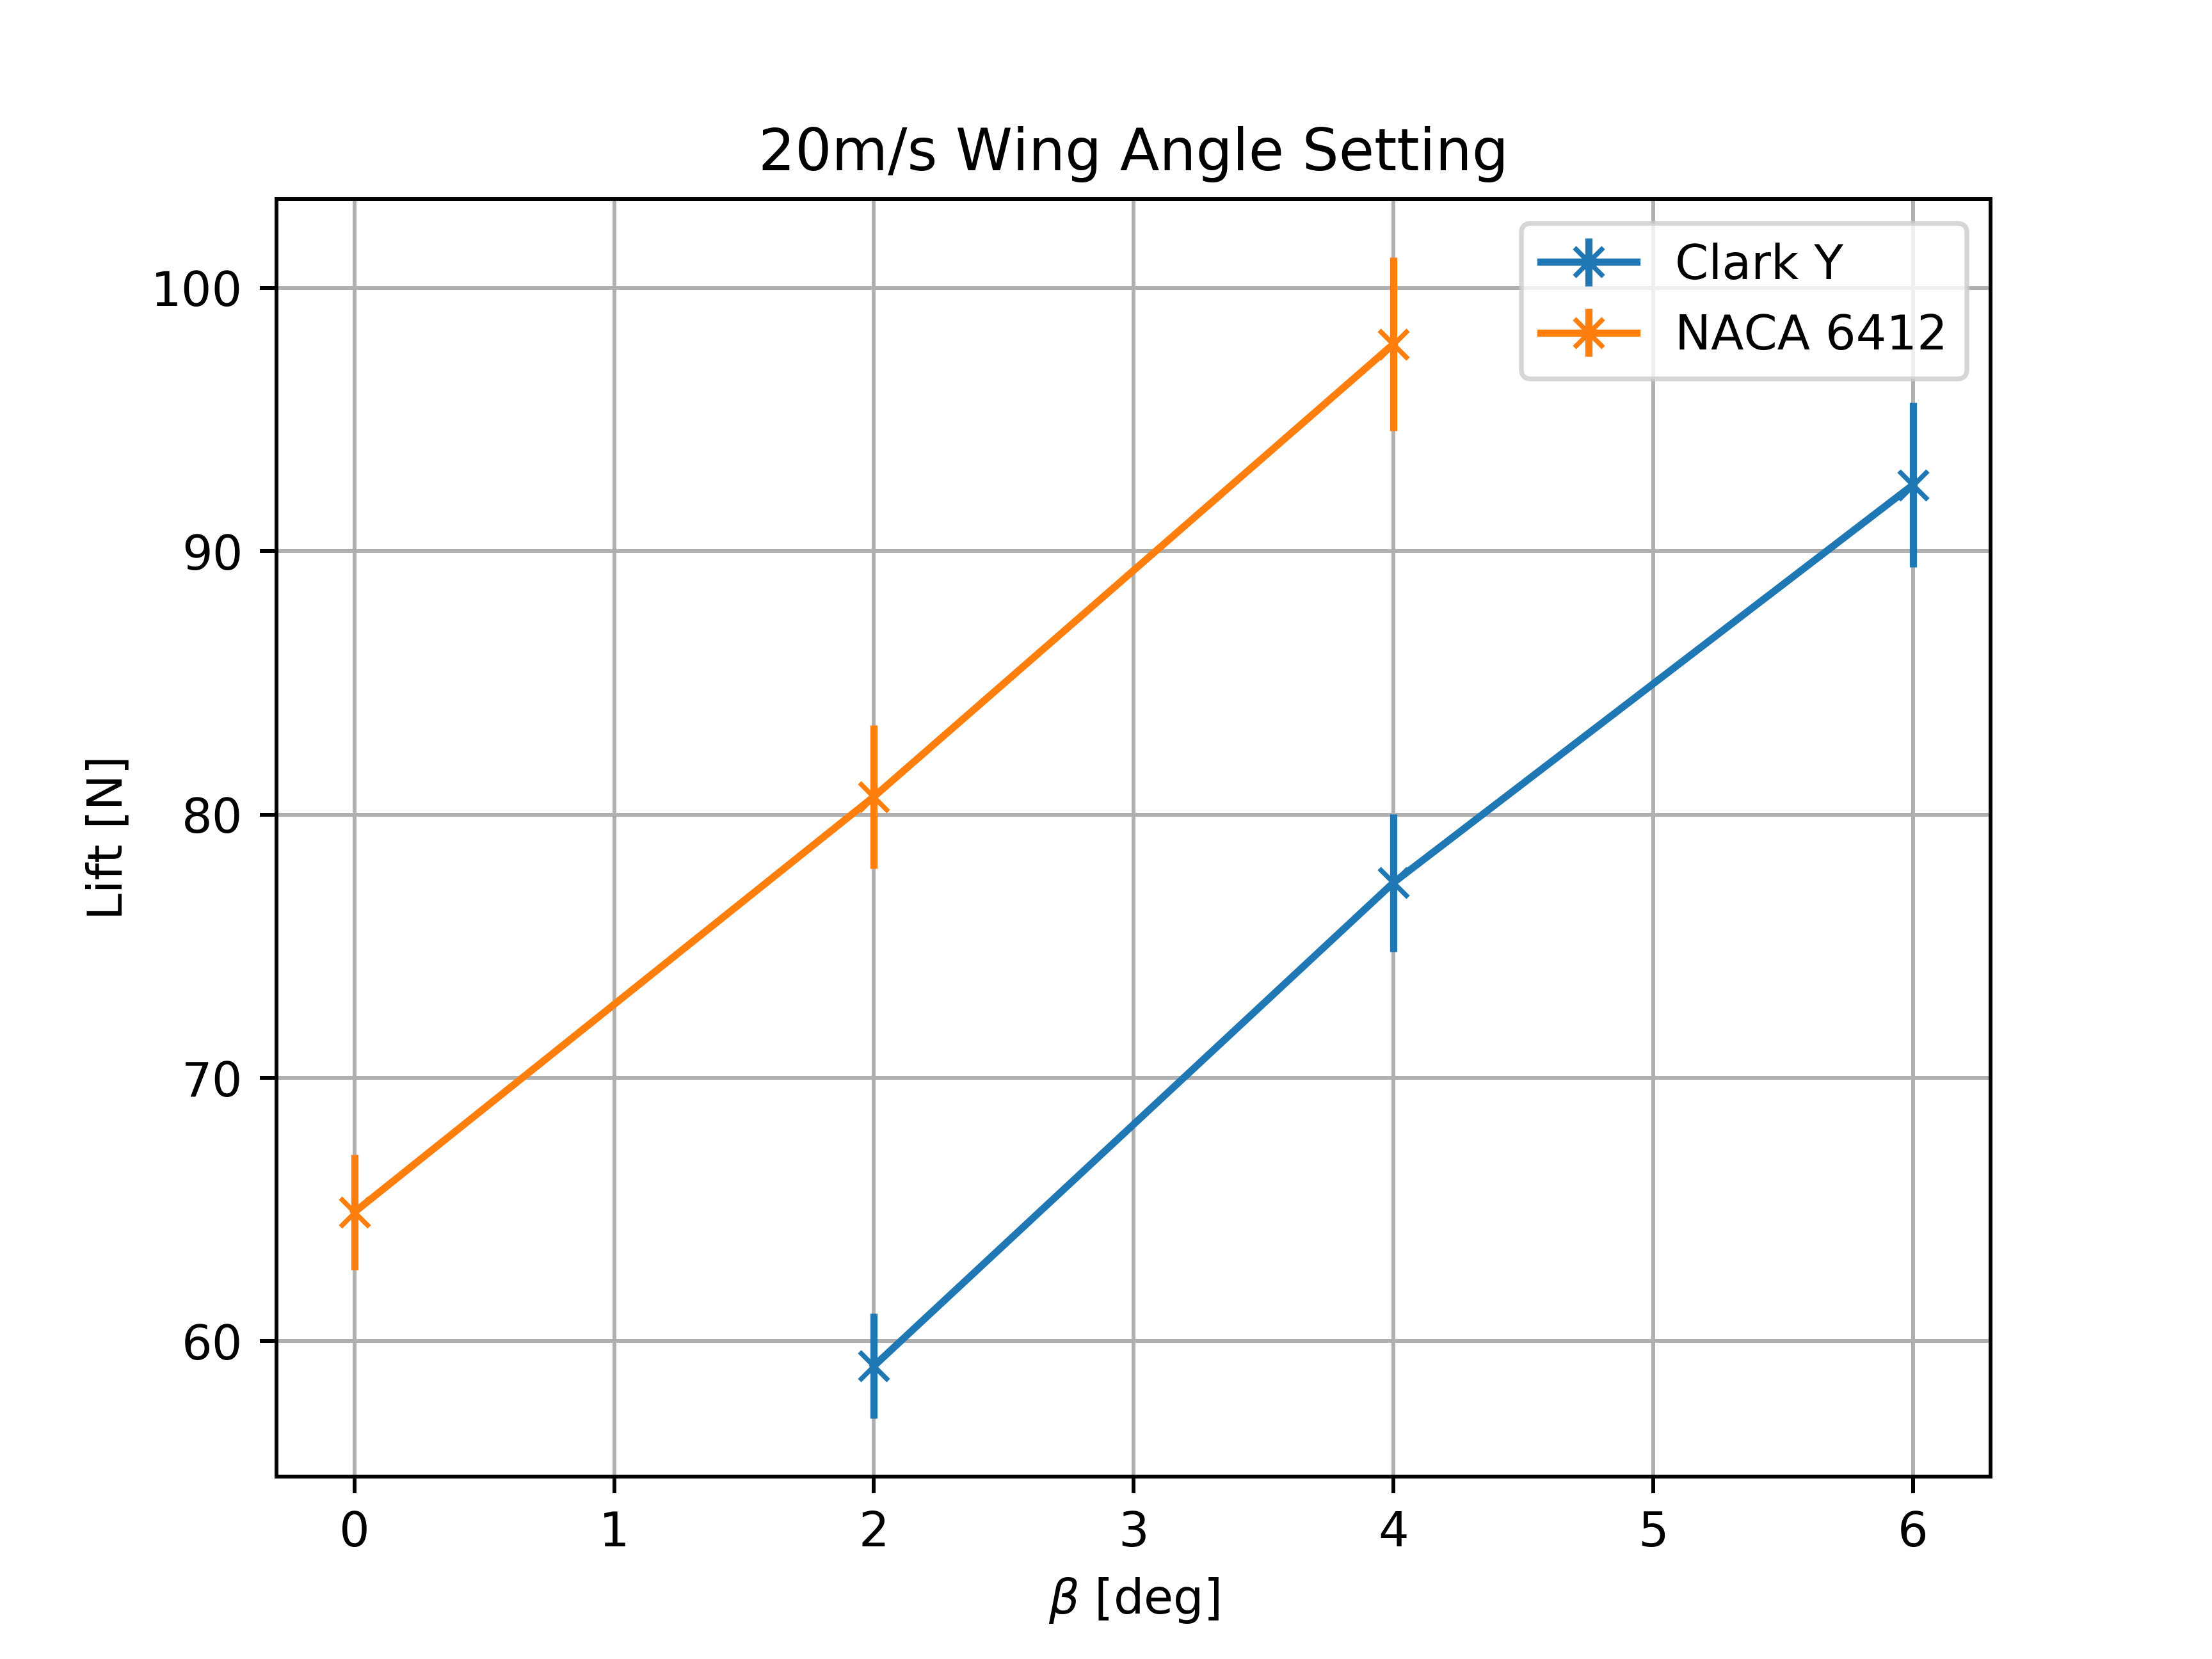
\includegraphics[width=\textwidth]{wing-setting-angle}
        \caption{Wing setting angle}
        \label{fig:wind-tunnel-results:wing-setting-angle}
    \end{subfigure}
    \hfill
    \begin{subfigure}[b]{0.49\columnwidth}
        \centering
        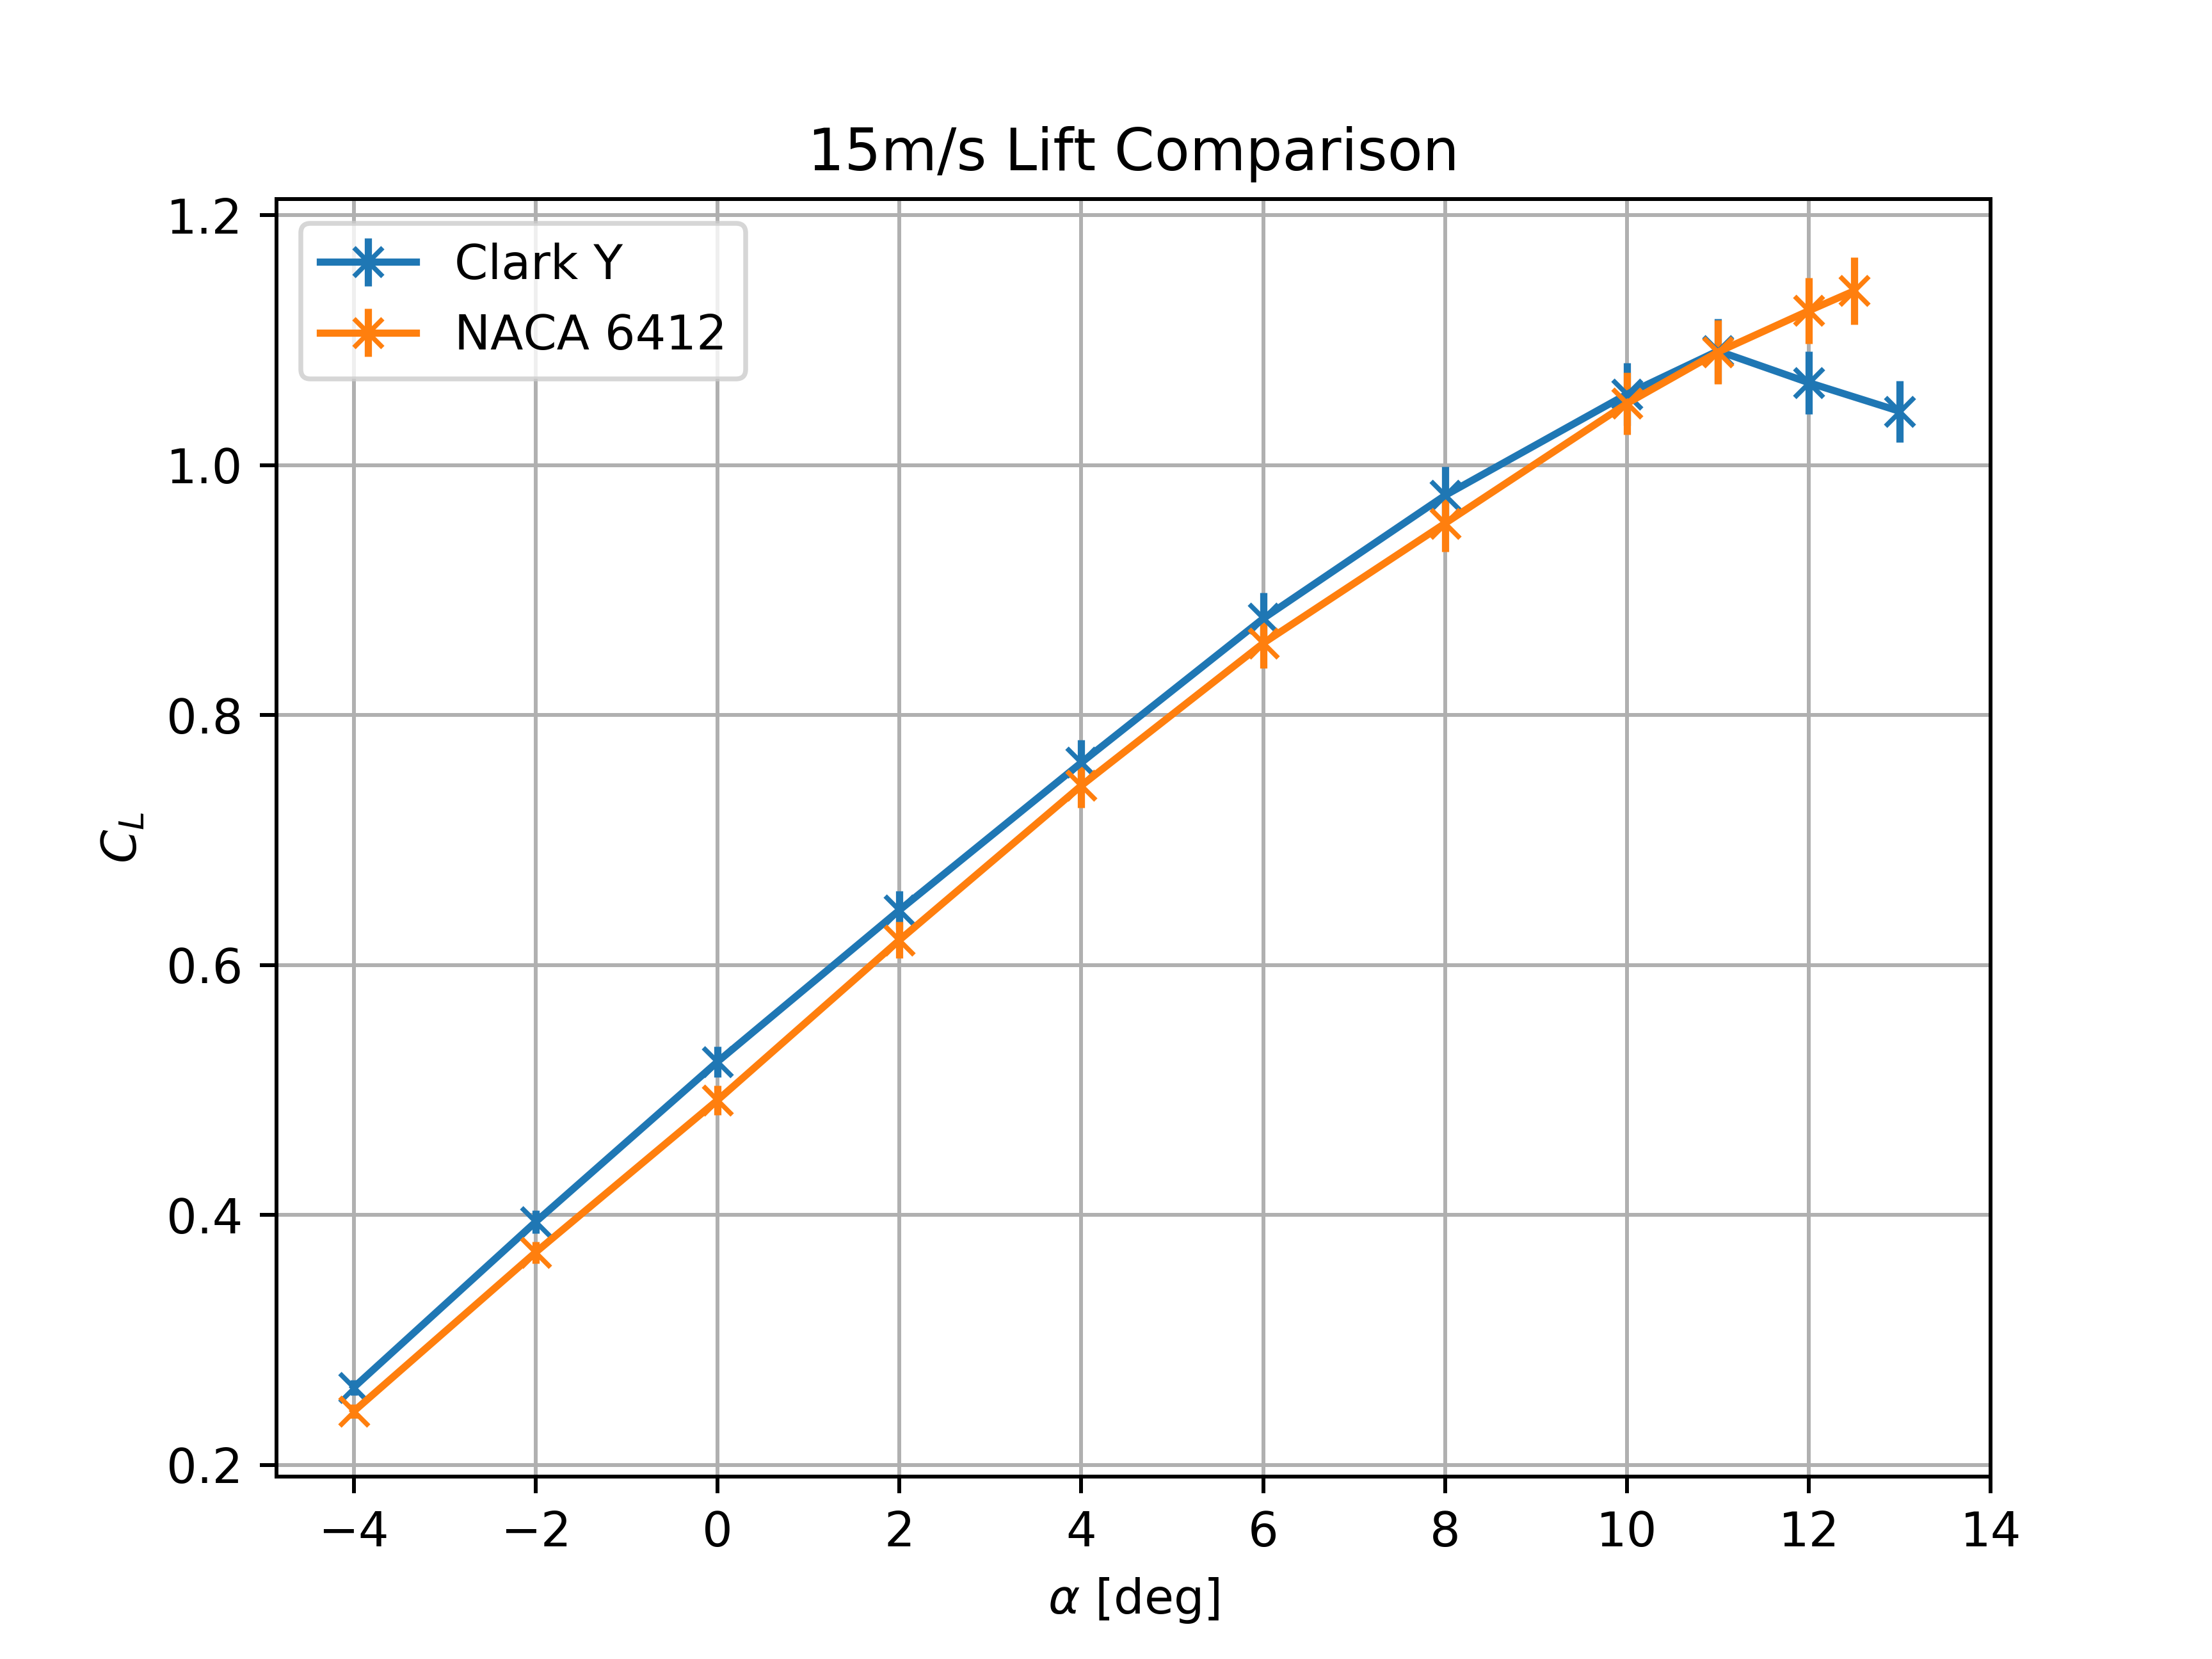
\includegraphics[width=\textwidth]{lift-comparison}
        \caption{Lift comparison}
        \label{fig:wind-tunnel-results:lift-comparison}
    \end{subfigure}

    \begin{subfigure}[b]{0.49\columnwidth}
        \centering
        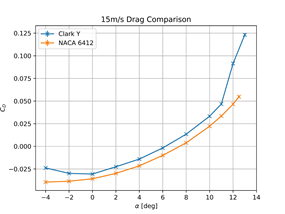
\includegraphics[width=\textwidth]{drag-comparison}
        \caption{Drag comparison}
        \label{fig:wind-tunnel-results:drag-comparison}
    \end{subfigure}
    \hfill
    \begin{subfigure}[b]{0.49\columnwidth}
        \centering
        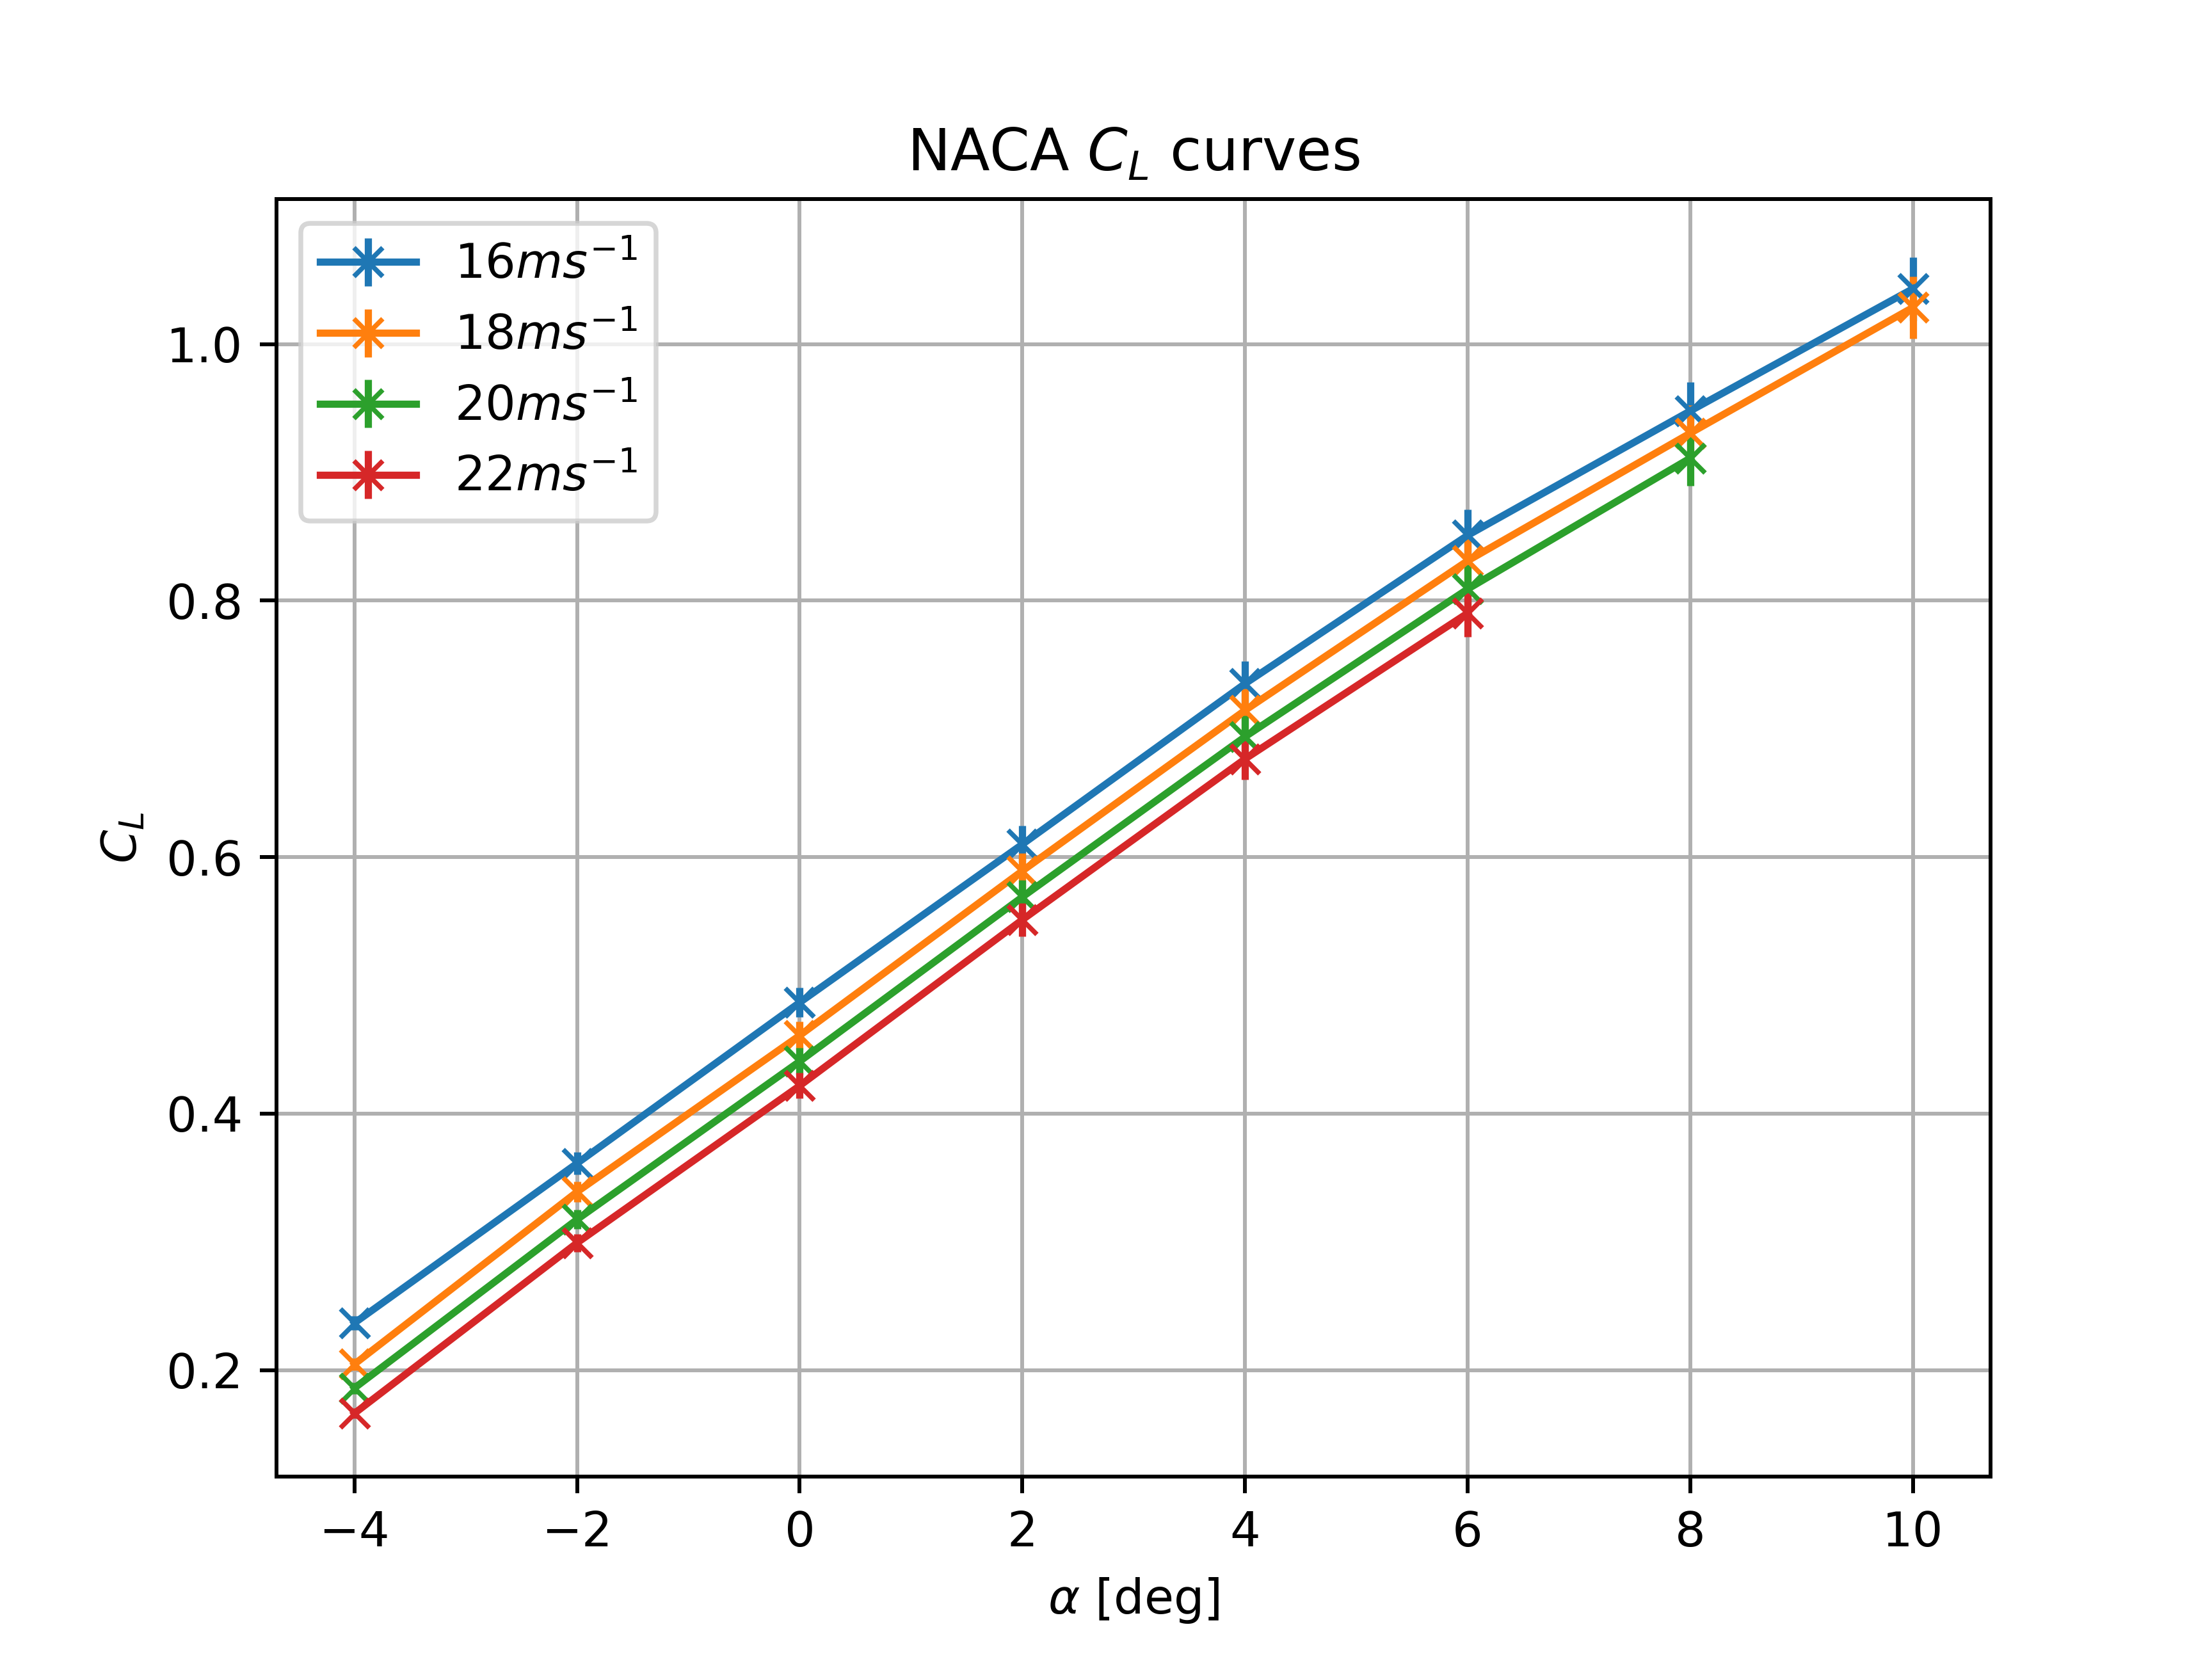
\includegraphics[width=\textwidth]{naca-lift-coefficient}
        \caption{NACA lift coefficient}
        \label{fig:wind-tunnel-results:naca-lift-coefficient}
    \end{subfigure}

    \begin{subfigure}[b]{0.49\columnwidth}
        \centering
        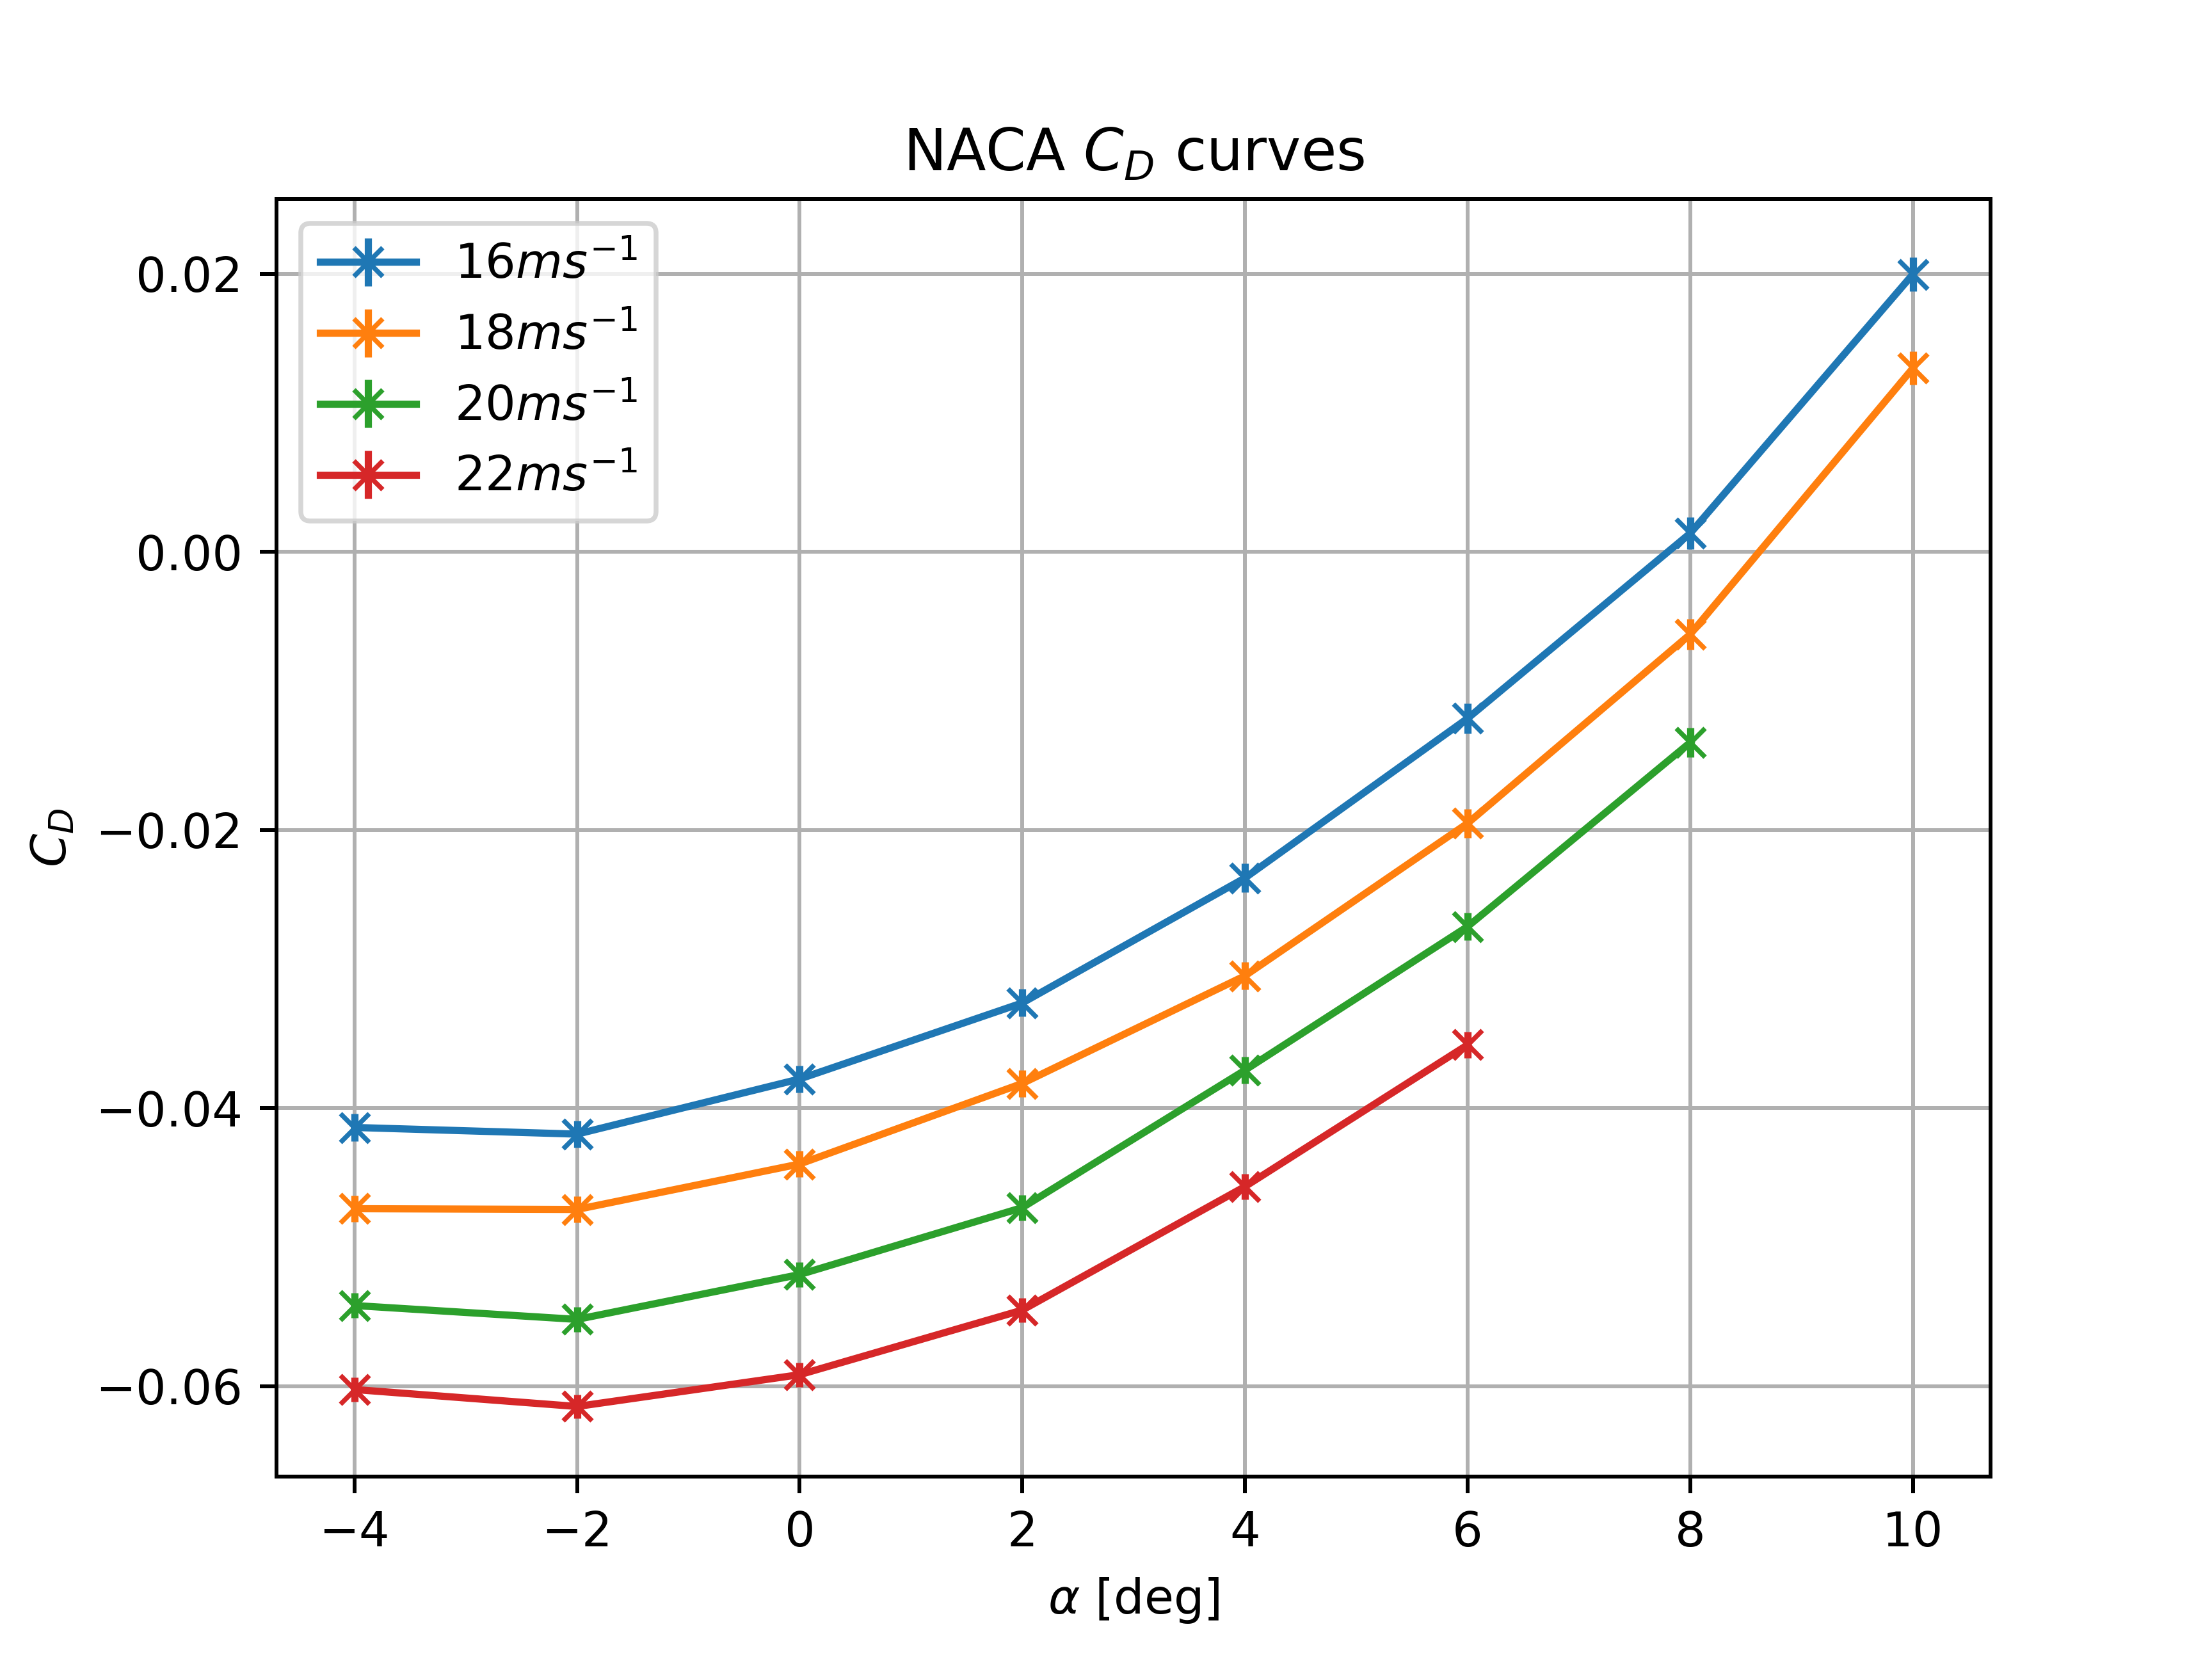
\includegraphics[width=\textwidth]{naca-drag-coefficient}
        \caption{NACA drag coefficient}
        \label{fig:wind-tunnel-results:naca-drag-coefficient}
    \end{subfigure}
    \hfill
    \begin{subfigure}[b]{0.49\columnwidth}
        \centering
        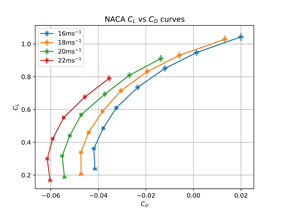
\includegraphics[width=\textwidth]{cl-against-cd}
        \caption{$C_L$ against $C_D$}
        \label{fig:wind-tunnel-results:cl-against-cd}
    \end{subfigure}

    \begin{subfigure}[b]{0.49\columnwidth}
        \centering
        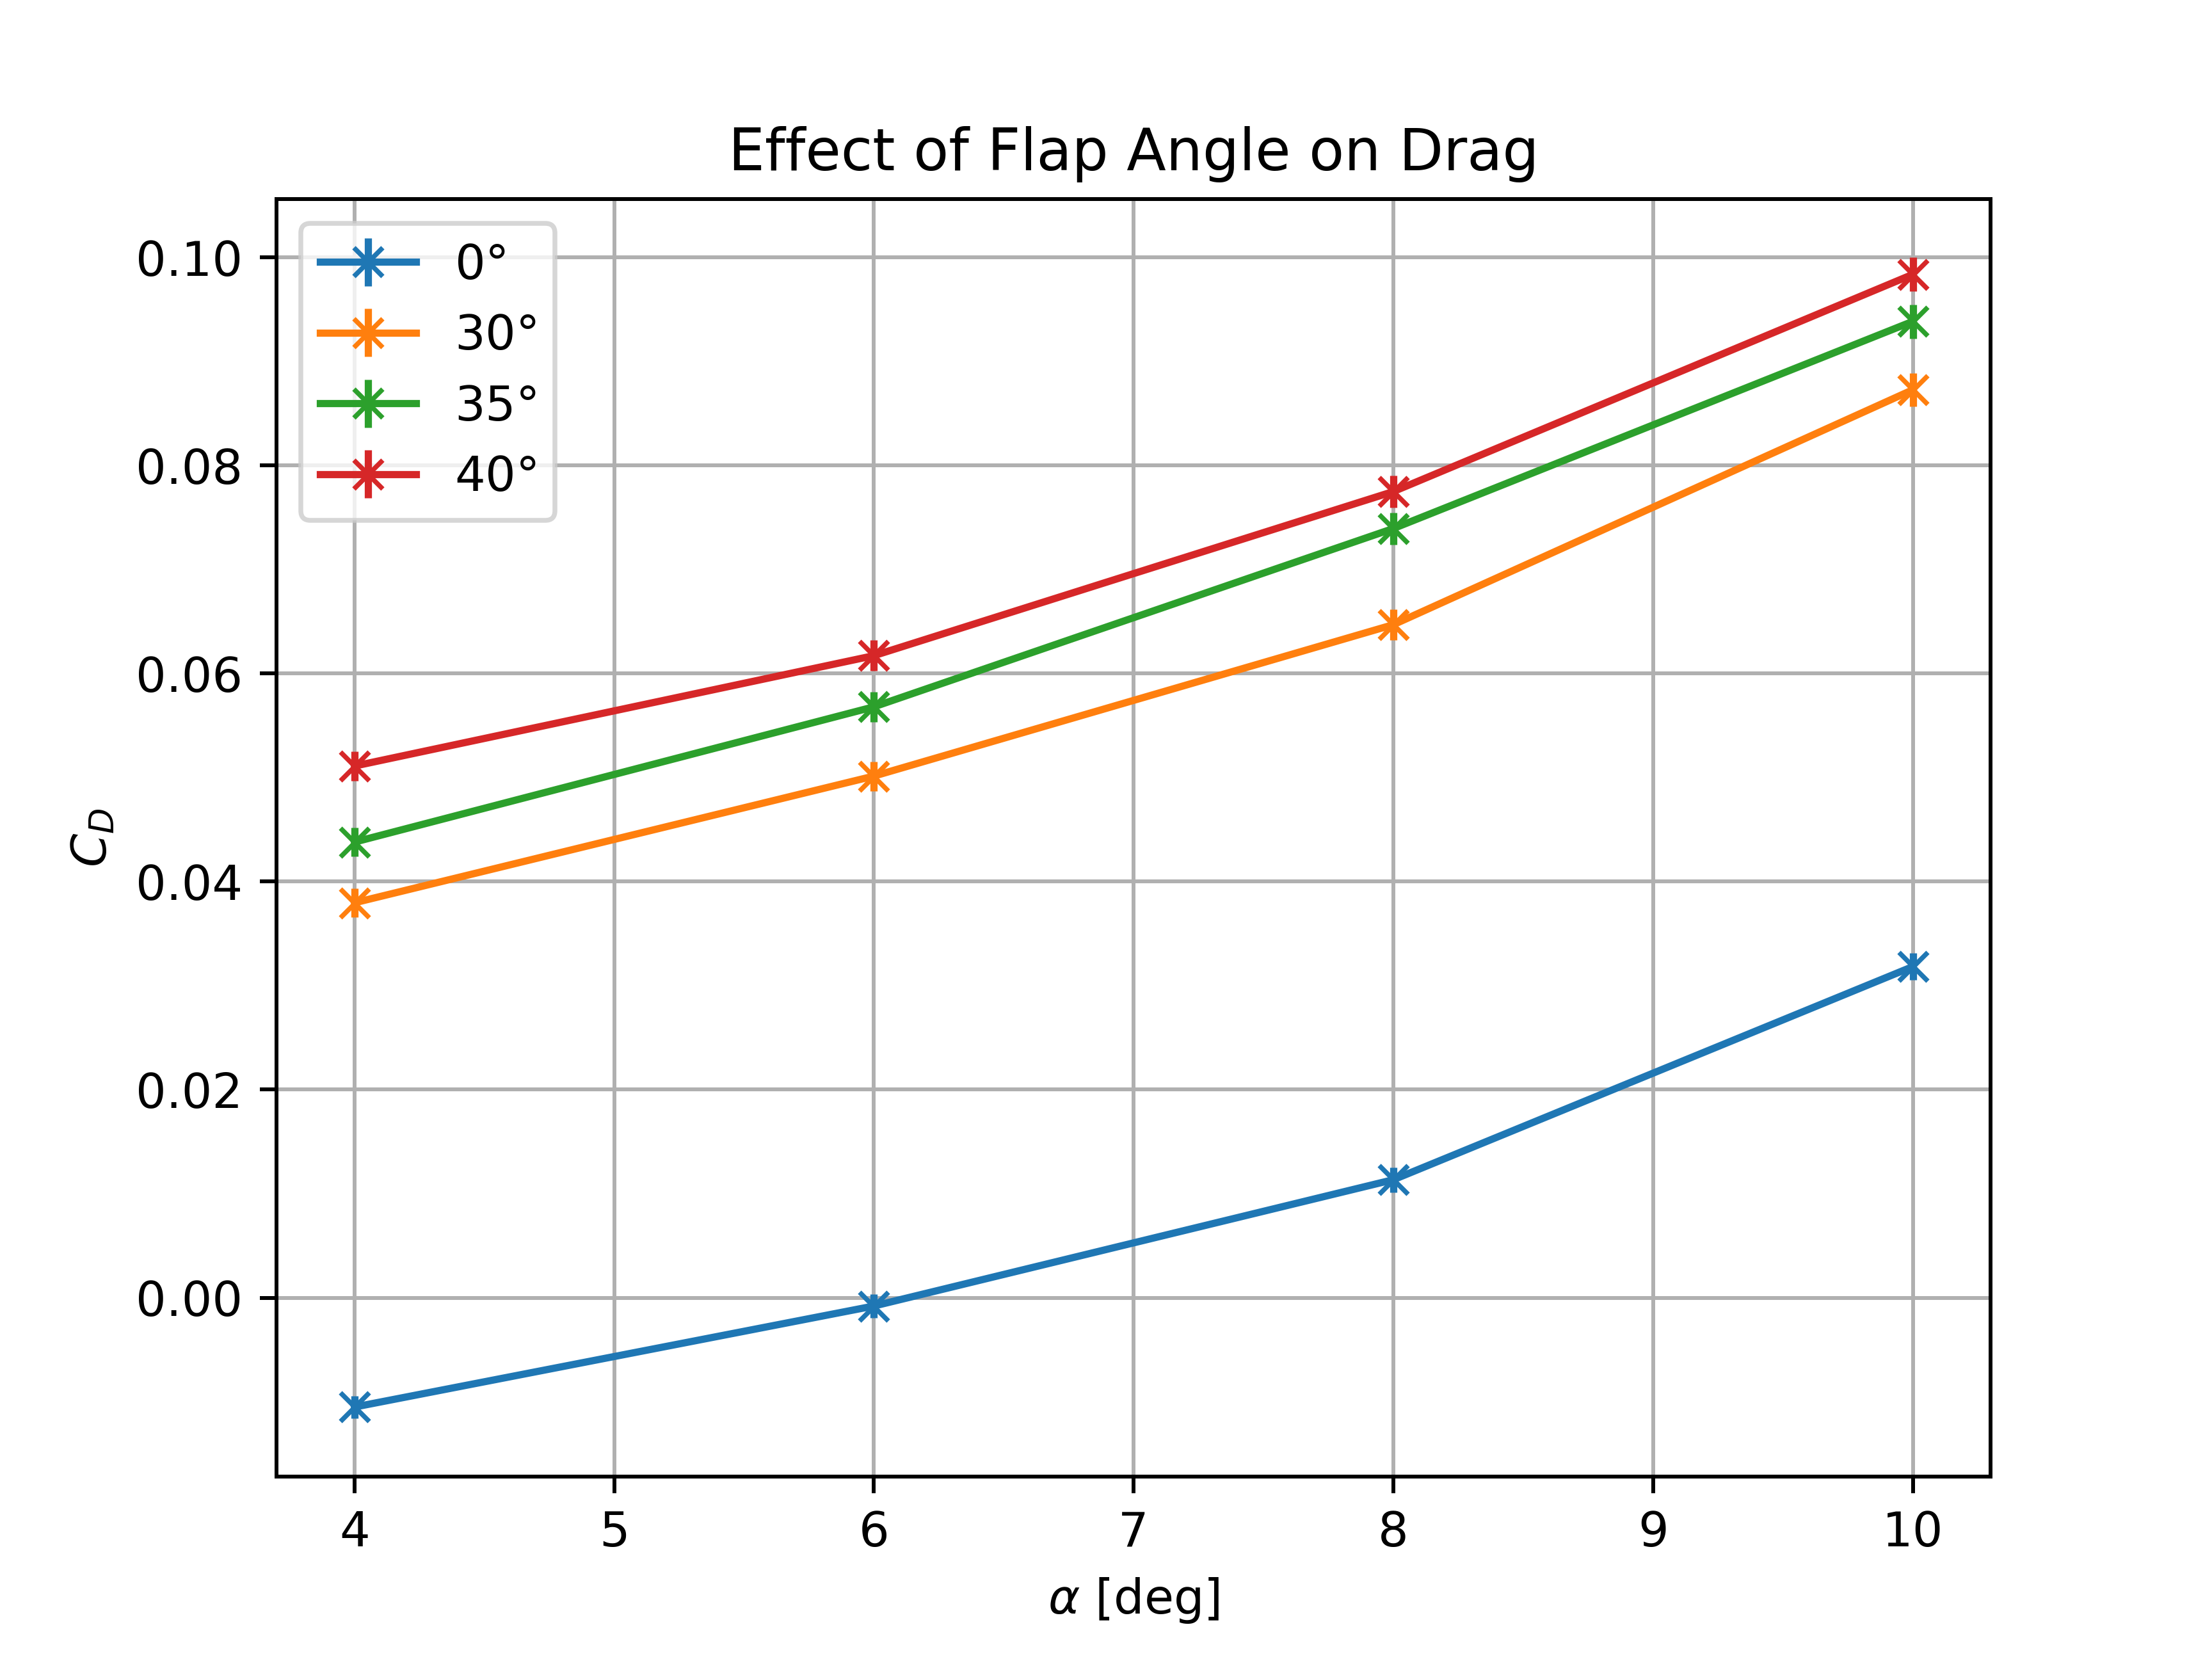
\includegraphics[width=\textwidth]{flap-drag-comparison}
        \caption{Flap drag comparison}
        \label{fig:wind-tunnel-results:flap-drag-comparison}
    \end{subfigure}
    \hfill
    \begin{subfigure}[b]{0.49\columnwidth}
        \centering
        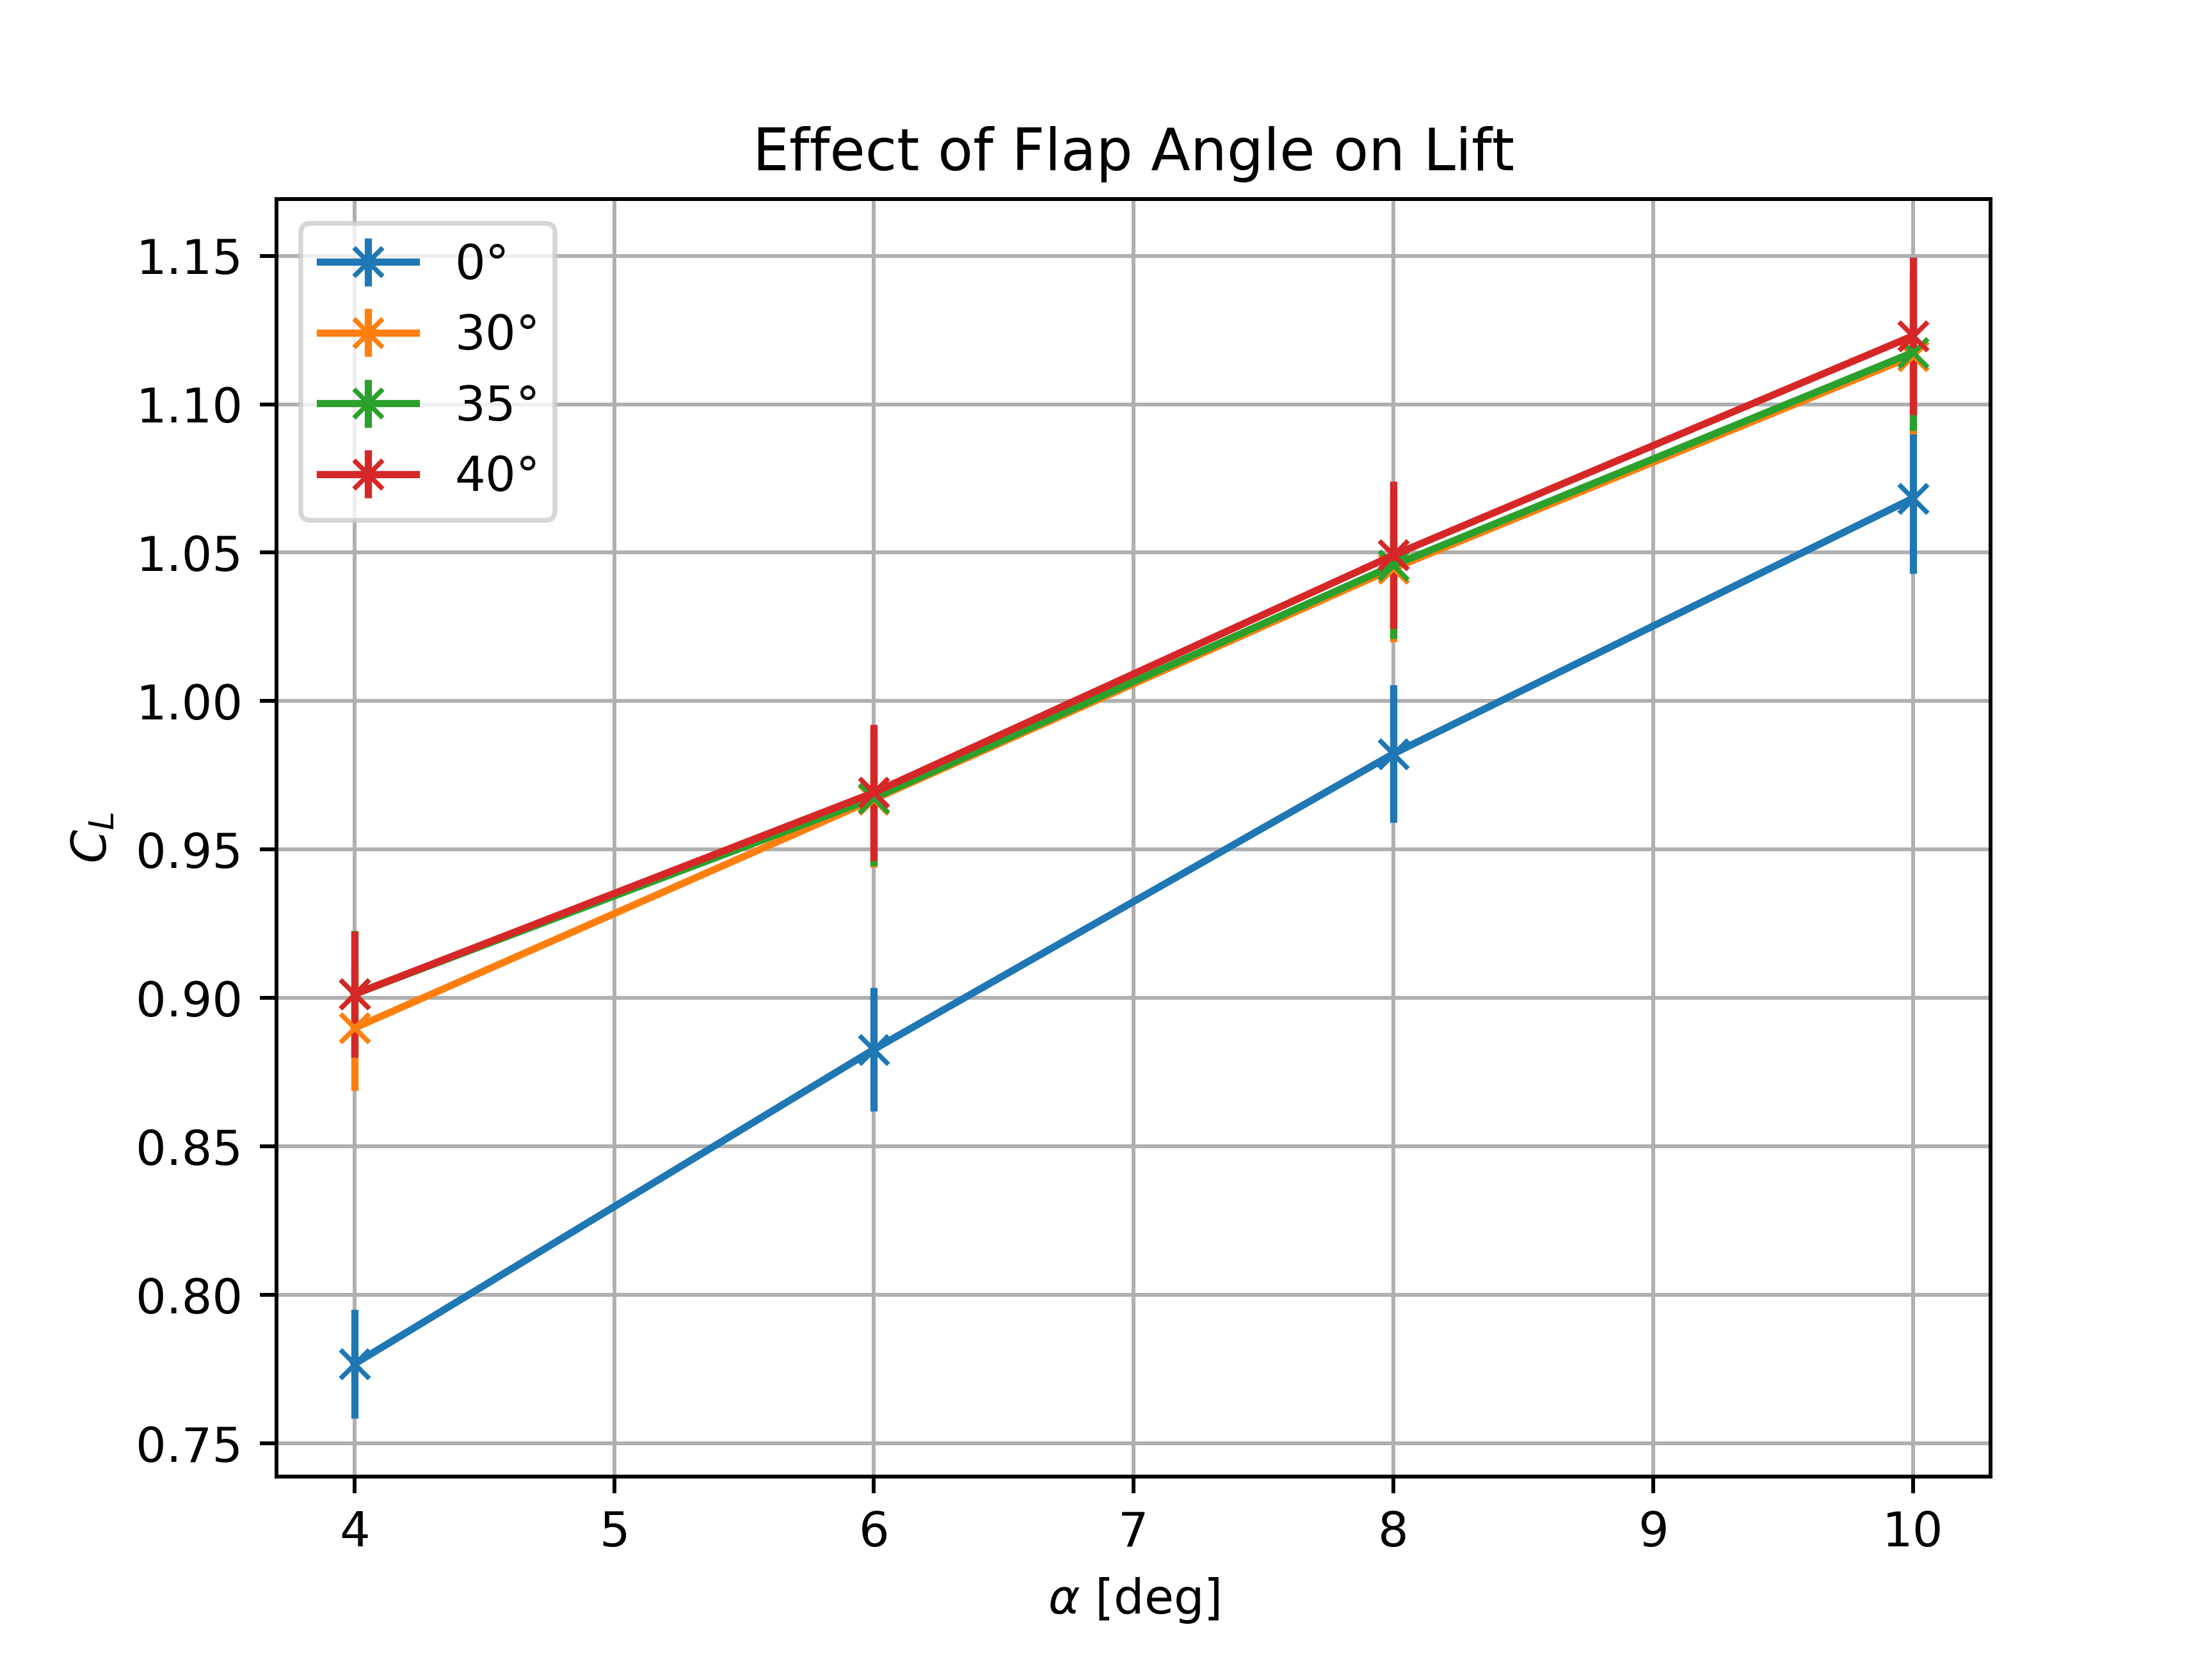
\includegraphics[width=\textwidth]{flap-lift-comparison}
        \caption{Flap lift comparison}
        \label{fig:wind-tunnel-results:flap-lift-comparison}
    \end{subfigure}

    \begin{subfigure}[b]{0.49\columnwidth}
        \centering
        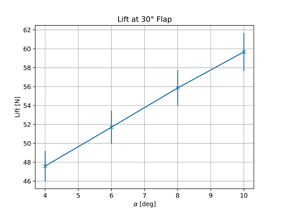
\includegraphics[width=\textwidth]{30-degree-flap-lift}
        \caption{30$^o$ flap lift}
        \label{fig:wind-tunnel-results:30-degree-flap-lift}
    \end{subfigure}
    \hfill
    \begin{subfigure}[b]{0.49\columnwidth}
        \centering
        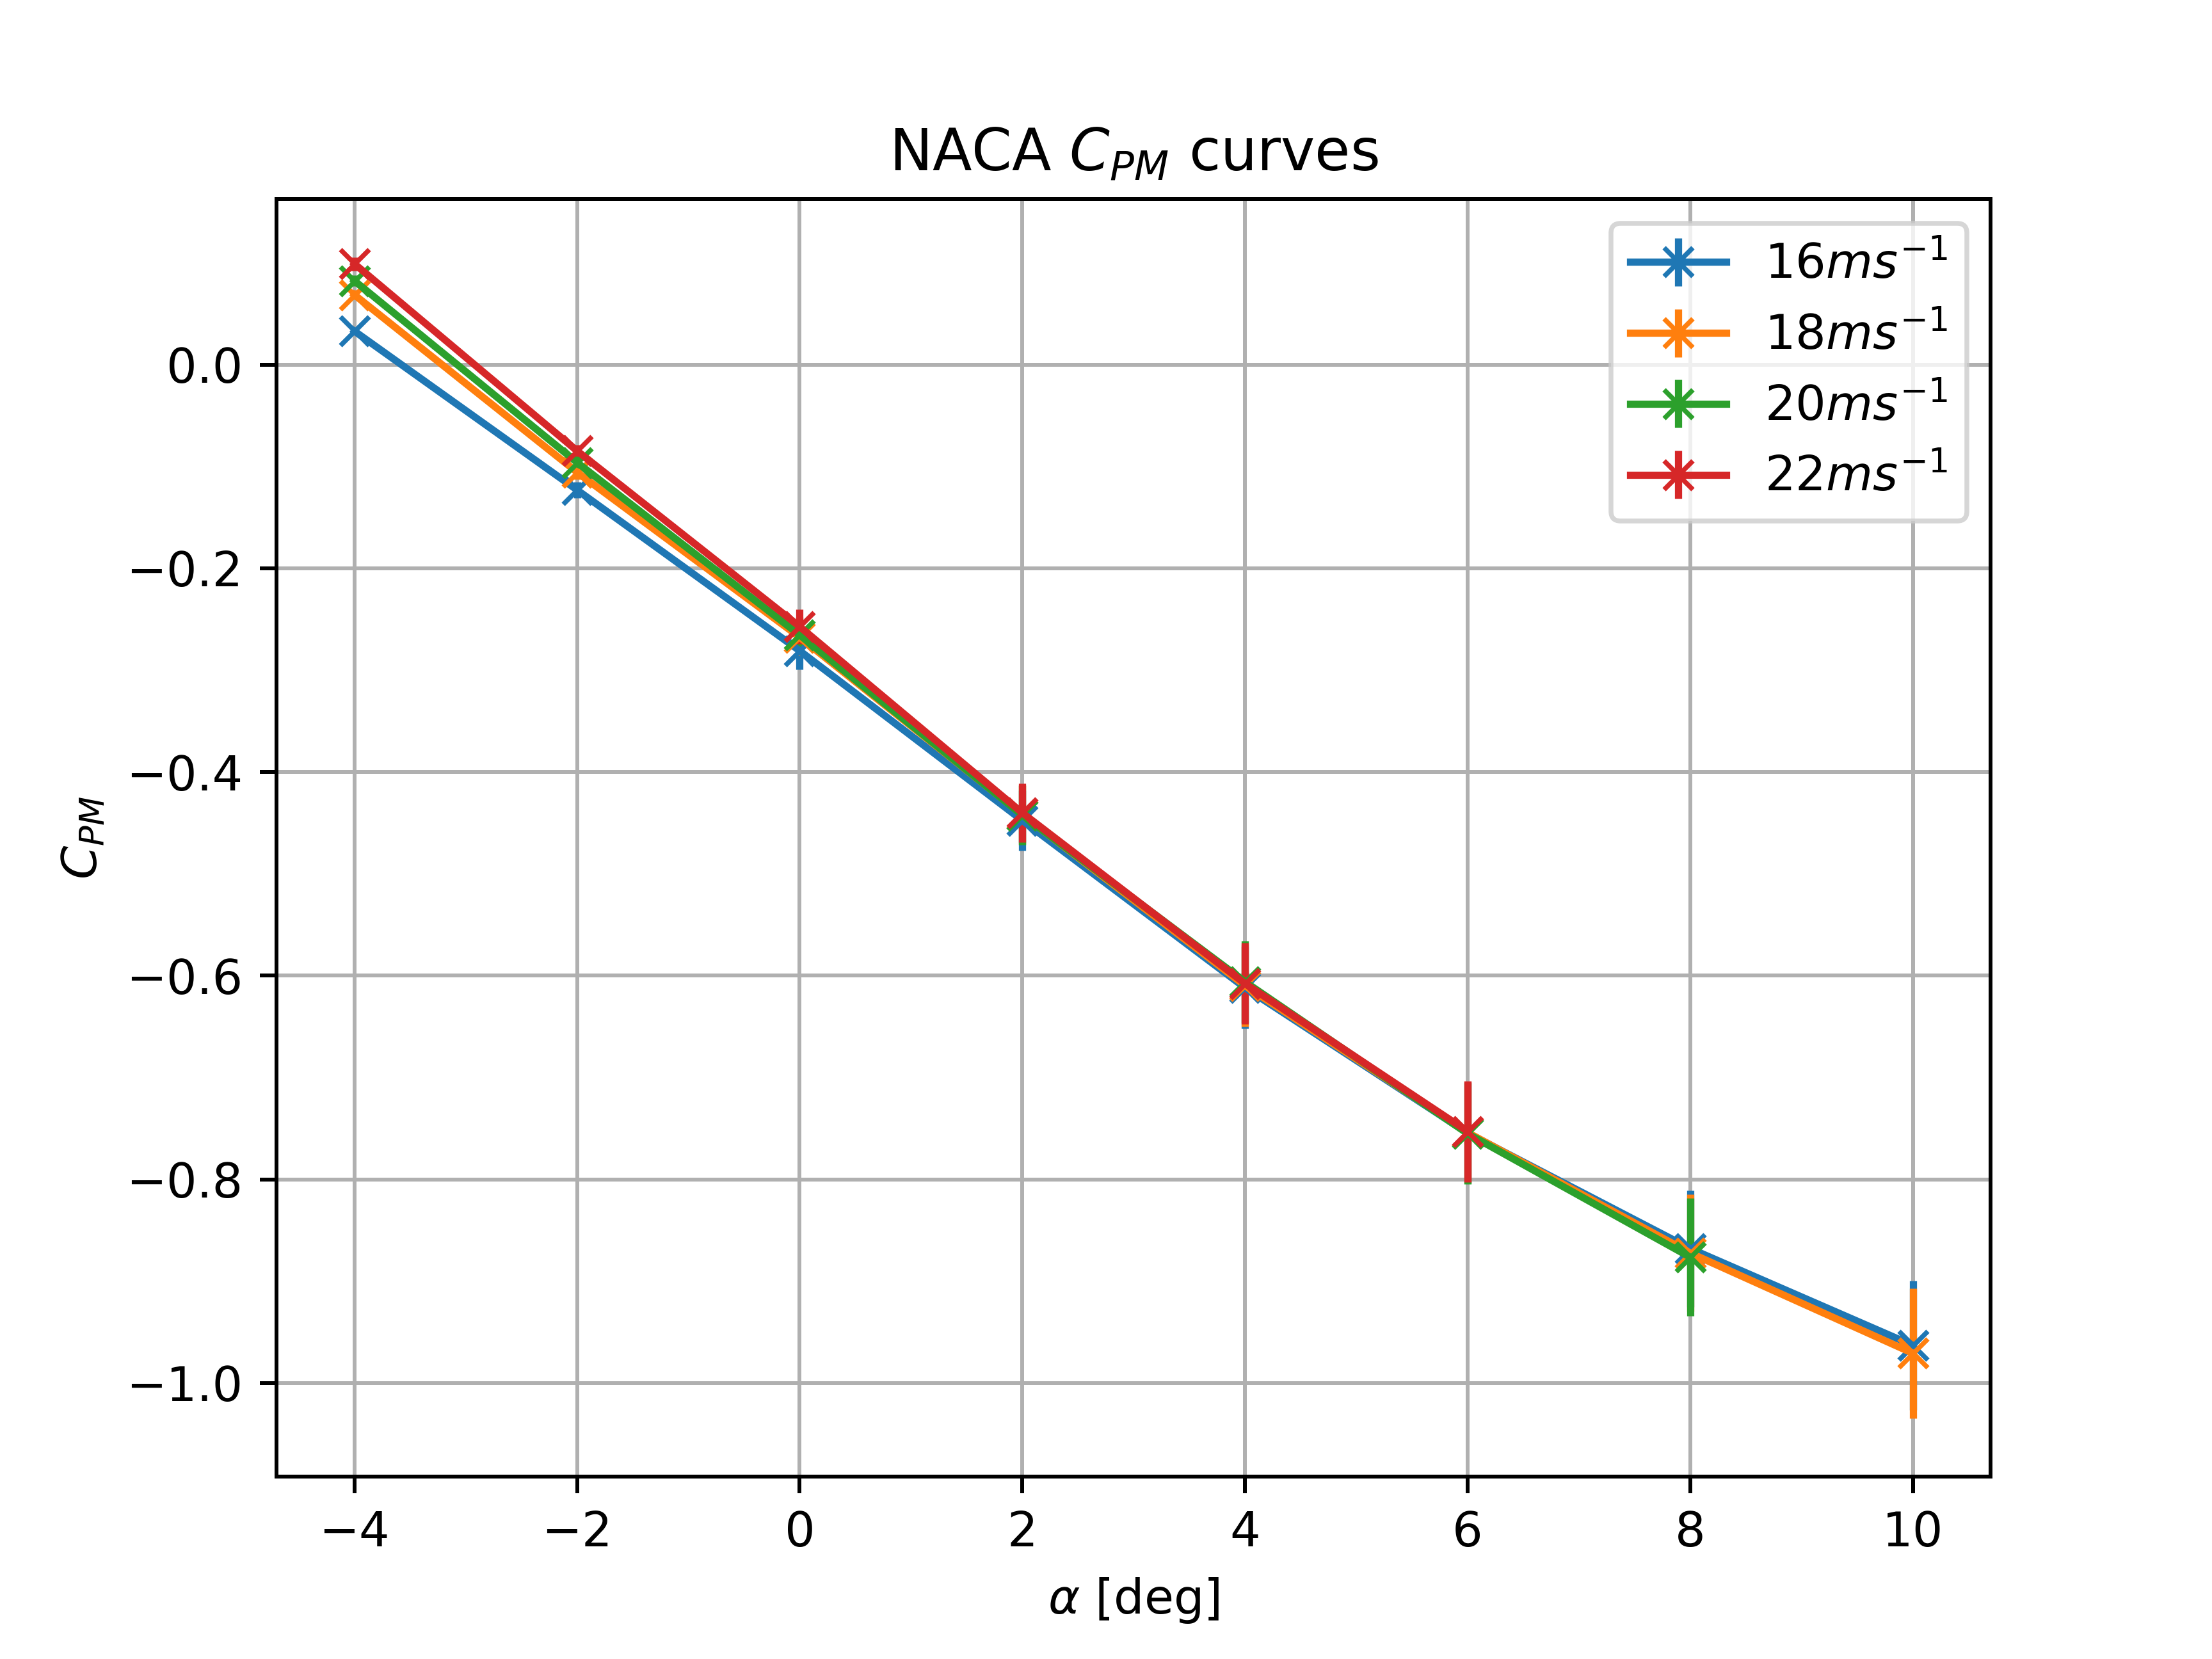
\includegraphics[width=\textwidth]{moment-coefficients}
        \caption{Moment coefficients}
        \label{fig:wind-tunnel-results:moment-coefficients}
    \end{subfigure}

    \caption{graphical results of the analysis of data gathered during the wind tunnel test.}
    \label{fig:wind-tunnel-results}
\end{figure}

The results from the wind tunnel test required considerable post processing before analysis could be carried out, but once this was complete the graphs could be made, and the results could be easily analysed.
There was a significant problem when the correction for the drag of the mounting structure, used to hold the model in the wind tunnel, was implemented because it caused some of the drag results to be negative.
This is a significant problem and means that the drag data is unreliable, however the trends seen in the results can still be useful.
The drag data will now rely on CFD and additional wind tunnel tests for clarification.
Figure 1 a) shows the results from the initial test carried out, where the setting angle of the two wings were found by increasing the angle of the wing against the fuselage until the lift exceeded the target weight of 70N at the target cruise speed of 20m/s.
This graph shows that the NACA 6412 exceeded this lift at 1, and so was set at 2 for the rest of the test to give a margin as the final wing is expected to produce slightly less lift due to the attachment of the propulsion units.
The Clark Y exceeded the required lift at around 3 and so was set at 4 for the same reason. 

Figure 1 b) and c) show the comparison between the NACA 6412 and Clark Y wings through a full sweep of angle of attack.
At this point the wing were set at their specified angles, and so the whole model was moved through the range of angles of attack to give the data.
It can be seen that the two wings produce very similar $C_L$ values, this is expected thanks to setting the wings at their respective angles, however the Clark Y aerofoil stalls before the NACA 6412, thus giving a lower maximum lift, and this is one of the reasons the NACA 6412 was chosen as the aerofoil for the final UAV instead of the Clark Y.
It can also be seen that the Clark Y has a higher $C_D$ at all angles of attack, and so is less efficient than the NACA 6412, and so the NACA 6412 was chosen. 

Figure 1 d) e) and f) show the plots for the wind tunnel model equipped with the NACA 6412 at a range of airspeeds showing the performance throughout the target flight envelope of the UAV.
Figure 1 d) shows that the $C_L$ remains almost constant as the airspeed changes, as expected as there are no compressibility effects as these speeds.
Figure 1 e) shows that the $C_D$ reduces with the increase in airspeed, this is due to the reduction of lift induced drag at higher speeds.
Figure 1 f) shows that therefore the highest aerodynamic efficiency is found at the highest tested speed of 22m/s, and although this speed is above the targeted cruise speed of the UAV, it shows that for maximum range, the UAV should be flown as fast as possible. 

Figure 1 g) and h) show the results of the flap test that was performed with the NACA 6412 wing.
Figure 1 g) shows the increase in $C_D$ that comes with each increase of the flap angle, and Figure 1 h) shows that the $C_L$ increases significantly with the flaps activated, but that the variation of the flap angle has little to no effect on the increase in $C_L$.
This suggests that the flaps are stalling at 30, and so the flap angle to be used in the final model will be 30.
Figure 1 i) shows that the lift increase was not enough to provide the required lift at the target take-off/landing speed of 12m/s, with the maximum lift produced being just under 60N at 10.
The wing has not stalled at this point and so there is possibility for the wing to produce more lift at a higher angle of attack, however this could not be tested as 10 was the highest angle that could be reached.
Even so, it is clear that the design of the flaps needs to be modified to improve their effectiveness, and also the area of the wing used for the flaps could be increased in order to maximise their effectiveness. 

The wind tunnel test also provided data for the pitching moment about the aerodynamic centre of the wing, as shown in Figure 1 j), which gives an insight into the aerodynamic stability of the model and the pitching moment developed by the wing.
The data shows that the coefficient of pitching moment is independent of airspeed, and that its negative at 0 angle of attack, which is not ideal as it means that the aircraft would want to pitch down and so the pilot would need to trim the model, or use constant elevator in order to fly level.
However the negative gradient of the line on the plot is good as this means that the aircraft is aerodynamically stable in pitch, so any pitching up of the aircraft would produce an increase in the pitching down moment and the aircraft would automatically stabilise.
Also, with an adjustment to the tail-plane, the magnitude of the pitching moment could be made zero at 0 angle of attack by producing a counteracting moment with an angled tail-plane, and then the pilot would not need to trim the aircraft by such a significant magnitude. 

The uncertainty of the results has been calculated for all results and is shown as vertical bars for every point on the plots in Figure 1.
The uncertainties were calculated using the know accuracies of the recorded results, as well as repeats performed during the testing.
The maximum number of repeats for one test was only 2, and so the sample size is not significant, but the uncertainties are still reasonably small even with a 95.45\% confidence.
These uncertainties were then converted to percentages and applied to all results of that type, with an example table for the uncertainty of $C_L$ shown in Table 1, and the others provided in the appendix. 

% TODO: insert table from &REF2
% TODO: units
% TODO: define uncertainty and variance outside table
% TODO: reduce width slightly
\importtable{|
    >{\raggedright\arraybackslash}m{0.16\columnwidth}
    >{\raggedleft\arraybackslash}m{0.16\columnwidth}
    >{\raggedleft\arraybackslash}m{0.17\columnwidth}
    >{\raggedleft\arraybackslash}m{0.17\columnwidth}
    >{\raggedleft\arraybackslash}m{0.17\columnwidth} |
}{
    \hline
    Measured variable & $L$ & $q$ & $S$ & Rep. $C_L$ \\
    \hline
    Typical value & 77.04 & 249.55 & 0.6 & 0.01715 \\
    Accuracy & 0.07704 & 0.349 & 0.0012 & 0.01213 \\
    PDF & rect. & rect. & rect. & norm. \\
    PDF factor & 1.7321 & 1.7321 & 1.7321 & 1 \\
    $k$ factor & 1 & 1 & 1 & 1 \\
    SC value & 0.006679 & -0.00206 & -0.85754 & 1 \\
    Uncertainty & 0.000297 & -0.000416 & -0.000594 & 0.012128 \\
    Variance & $9\times10^{-8}$ & $1.7\times10^{-7}$ & $3.5\times10^{-7}$ & $1.471\times10^{-4}$ \\
    \hline
}{uncertainty calculations for $C_L$.}{cl-uncertainty}

\importtable{| l r |}{
    \hline
    Combined standard uncertainty & 0.01215 \\
    $C_L$ mean & 0.5145 \\
    Percentage uncertainty & 2.36 \\
    \hline
}{uncertainty summary for $C_L$.}{uncertainty-summary}

Unfortunately, the scope of the work required to design a fully functional tailplane with control surfaces had not been realised at this point, and the design was far too simple, with no mounting angle or control surfaces.
The tail was also undersized based on observation by our project supervisors.
Because of this, little work went into analysing the results from this test in terms of the tailplane, and work on the next version essentially started from scratch. 

\subsection{Motor and propellor test} \label{sec:design-process:interim-design-review:motor-and-propellor-test}

\subsubsection{Overview} \label{sec:design-process:interim-design-review:motor-and-propellor-test:overview}

\importimage{motor-bracket}{the motor bracket attached to the rear of the motor.}{Motor bracket}{0.5}
\importimage{motor-test}{the motor in the wind tunnel.}{Motor test}{0.5}

Once the motor and propeller selection had been completed based on wind tunnel results and propeller performance analysis, we ordered one of the wing motors with its tractor configuration propeller in order to test them together.
This test was to be performed in a small wind tunnel so as to give data for the motor in flight as well as a static thrust test.
The motor mount is a load cell located at the centre of the wind tunnel section, as shown in Figure 1 b), and to attach the motor a bracket is required.
The main part of this bracket had already been made for the testing of a different motor by the university, and so only a small plate was required to mount our motor to the existing setup.
This mount was made from aluminium sheet to fit to the back of the motor and mount onto the load cell, and is shown in Figure 1 a).
It required some precision marking and drilling for the outer holes as there were tight tolerances on the bracket it was to attach to, while the motor holes could be slightly less precise due to the countersunk bolts holding it in place.
A central clearance hole was required to allow the motor shaft to pass through, into the void created by the existing bracket in order to avoid the motor shaft hitting against the load cell.
The tests carried out were at wind speeds of 0m/s, 10m/s, and 15m/s, and at each wind speed the voltage was held at around 14.9V representing a partially drained battery, and the current was varied from 0 to 22A, giving a range of RPM at which we collected the thrust and torque data up to a max power of 330W.
The RPM was measured from the input to the motor, rather than directly from the blades, because the blades of the propeller were too short to reach in front of the laser.
However, this RPM data is accurate enough for this experiment.
The load cell used to mount the motor formed a blockage in the wake of the propeller, and so this will have affected the results, however the effect of this was reduced as much as possible by manufacturing the bracket to be as small as possible.
Also, the motor when attached to the model will have the blockage of the wing and the power unit housing behind it, so this effect is a good representation of the motor in flight.
Additionally, in order to maximise the performance of the propeller, it was sanded before the test to remove any manufacturing defects and to ensure a smooth surface for the airflow.
The propeller was balanced by the manufacturer, and during the test showed no significant signs of imbalance, with the output data remaining smooth throughout the test showing no signs of large vibrations. 

\subsubsection{Results and analysis} \label{sec:design-process:interim-design-review:motor-and-propellor-test:results-and-analysis}

\importimage{manufacturer-comparison}{comparison between the power data quoted by the manufacturer and the data collected in the wind tunnel.}{Manufacturer comparison}{0.8}

Figure 1 shows that the data provided by the propeller supplier and the data from the test performed match up very well for the power output from the propeller at a given RPM, this shows that the data provided is accurate and can be used as a good estimate of the power provided by the other propellers intended for use on the UAV, the pusher version of the propeller tested and both fuselage propellers. 

\importimage{thrust-data}{thrust data collected at the three airspeeds tested.}{Thrust data}{0.8}

Figure 2 shows again the similarities between the data given by the propeller supplier for the static case and the test data, but more importantly this graph shows the drop off of thrust with an increase in airspeed.
This can be used to estimate the thrust developed by the propulsion unit at cruise, and so find if the propeller is suitable for use.

\importimage{maximum-thrust}{maximum thrust at the airspeeds tested, with an extrapolation to the intended cruise speed of 20 m.s-1}{Maximum thrust}{0.8}

Figure 3 shows the extrapolation of the thrust of the propulsion unit at different airspeeds up to the intended cruise speed of 20m/s.
This predicts that the thrust in cruise would be 6.5N, therefore 13N for the total thrust of the UAV.
From CFD drag results giving 10N at 20m/s, this would be sufficient to cruise at 77\% throttle, saving battery and giving a longer flight time than if cruise had required full throttle. 

\importimage{efficiency-data}{efficiency data collected at the three different airspeeds tested}{Efficiency data}{0.8}

Figure 4 shows the efficiency curves for the power unit at different airspeeds, and also the data provided by the supplier for the propeller at static conditions.
From this data it is clear to see a significant difference between the data provided by the propeller manufacturer and the data recorded, which is surprising given that the power produced by the propeller is so similar to the manufacturer data.
This suggests that the difference is due to the motor used, and so suggests that the motor is providing a significant loss of power in the system.
If the difference is assumed to be entirely due to the motor, we can apply this back to the other airspeed cases to find the propeller efficiencies in these cases, this is assuming that the motor efficiency is not affected by the airspeed, only by its RPM.
This assumption would not be entirely accurate as the cooling would have an effect on performance, as well as the difference in drag on the rotating shell of the motor at different airspeeds.
However this effect is not important as the data needed is of the efficiency of the motor and propeller together, as is shown in the graph above, this data was then used to further update the constraint analysis and ensure that the power requirements were still met. 

\importimage{thrust-comparison}{comparison of thrust generated for a given input power at different airspeeds.}{Thrust comparison}{0.5}

Figure 5 shows how the effect of the motor efficiency lowers the thrust at a given input power.
This is due to the RPM of the propeller being lower for a given input power in the test than in the manufacturer data.
Also, this graph shows that the relationship between the thrust and the input power is tending towards an approximately liner relationship, and so the assumption that this is linear is a sensible one to make when updating battery life calculations.
Using this and the 77\% of max thrust required in cruise calculated earlier, we can assume that the power draw will be 77\% of the max, therefore giving an estimate battery life of just over 9 minutes if the power draw is constantly at this level, and so the flight time would be limited to 7 min for safety in order to ensure that the power does not cut off mid-flight. 

\end{document}
